%%%%%%%%%%%%%%%%%%%%%%%%%%%%%%%%%%%%%%%%%%%%%%%%%%%%%%%%%%%%%%%%%%%%%%%%%%%%%%%%
%                                                                              %
% Purpose:       Dense Three Column Summary                                    %
%                                                                              %
% Author:        Mark Kurzeja                                                  %
% Contact:       mtkurzej@umich.edu                                            %
% Client:        Mark Kurzeja                                                  %
%                                                                              %
% Code creation: 2015-10-10                                                    %
%                                                                              %
% Comment:       Create three column dense info sheets for the presentation o  %
%                f concise information or to quickly condense a topic or a     %
%                class into a handout                                          %
%                                                                              %
% License:       MIT Open Source License                                       %
%                                                                              %
%%%%%%%%%%%%%%%%%%%%%%%%%%%%%%%%%%%%%%%%%%%%%%%%%%%%%%%%%%%%%%%%%%%%%%%%%%%%%%%%

\documentclass[landscape]{article}
%opening
\title{}
\author{}
\usepackage{multicol}
% Control the geometry of the page with 1/2 inch margins
\usepackage[width = 10.5in, height = 8in]{geometry}
\usepackage{kpfonts}
%\usepackage{libertine}
%\renewcommand{\familydefault}{\sfdefault}
\usepackage{xspace}
\usepackage{nicefrac}
\usepackage{amsmath}
\usepackage{lipsum}
\usepackage{amsfonts}
\usepackage{graphicx}
\usepackage{wasysym} % Fullmoon
\usepackage{float}
\usepackage{todonotes}
\usepackage{booktabs}
\usepackage{amssymb}
\usepackage{makecell} % for \makecell{.... \\ .....} for multiline cells
\usepackage{changepage}   % for the adjustwidth environmen
\usepackage{siunitx} % For the num operator in producing scientific notation
\usepackage{multicol}

% For collapsing the lists to a single condensed itemized list
\usepackage{enumitem}
\setlist{nosep} % or \setlist{noitemsep} to leave space around whole list

% Specific functions that remove the issues with the spacing around an align enviroment
\usepackage{etoolbox}
\newcommand{\zerodisplayskips}{%
	\setlength{\abovedisplayskip}{2pt}%
	\setlength{\belowdisplayskip}{2pt}%
	\setlength{\abovedisplayshortskip}{2pt}%
	\setlength{\belowdisplayshortskip}{2pt}}
\appto{\normalsize}{\zerodisplayskips}
\appto{\small}{\zerodisplayskips}
\appto{\footnotesize}{\zerodisplayskips}

% ==============================================================================
% Listings Declaration
% ==============================================================================

\usepackage{listings} 
%\lstset{language=R} 
\usepackage{color}
\definecolor{mygreen}{rgb}{0,0.6,0}
\definecolor{mygray}{rgb}{0.5,0.5,0.5}
\definecolor{mymauve}{rgb}{0.58,0,0.82}

\lstset{ %
	backgroundcolor=\color{white},   % choose the background color; you must add \usepackage{color} or \usepackage{xcolor}
	basicstyle=\scriptsize,        % the size of the fonts that are used for the code
	breakatwhitespace=false,         % sets if automatic breaks should only happen at whitespace
	breaklines=true,                 % sets automatic line breaking
	captionpos=b,                    % sets the caption-position to bottom
	commentstyle=\color{mygreen},    % comment style
	deletekeywords={...},            % if you want to delete keywords from the given language
	escapeinside={\%*}{*)},          % if you want to add LaTeX within your code
	extendedchars=true,              % lets you use non-ASCII characters; for 8-bits encodings only, does not work with UTF-8
	frame=single,	                   % adds a frame around the code
	keepspaces=true,                 % keeps spaces in text, useful for keeping indentation of code (possibly needs columns=flexible)
	keywordstyle=\color{blue},       % keyword style
	language=R,                 % the language of the code
	otherkeywords={*,...},            % if you want to add more keywords to the set
	numbers=left,                    % where to put the line-numbers; possible values are (none, left, right)
	numbersep=5pt,                   % how far the line-numbers are from the code
	numberstyle=\tiny\color{mygray}, % the style that is used for the line-numbers
	rulecolor=\color{black},         % if not set, the frame-color may be changed on line-breaks within not-black text (e.g. comments (green here))
	showspaces=false,                % show spaces everywhere adding particular underscores; it overrides 'showstringspaces'
	showstringspaces=false,          % underline spaces within strings only
	showtabs=false,                  % show tabs within strings adding particular underscores
	stepnumber=1,                    % the step between two line-numbers. If it's 1, each line will be numbered
	stringstyle=\color{mymauve},     % string literal style
	tabsize=2,	                   % sets default tabsize to 2 spaces
	title=\lstname                   % show the filename of files included with \lstinputlisting; also try caption instead of title
}

% ==============================================================================
% Commands Declaration
% ==============================================================================

% A simple figure environment for inserting a picture into the column
% Arguments:
% 1: Name of the picture file
% 2: Caption for the picture
\newcommand{\qpics}[2]{
\begin{figure}[H]
\centering
\includegraphics[width=0.6\linewidth]{./#1}
\label{fig:#1}
\end{figure}
}

% Command for creating a very specific spaced hrule that wont interfere with the 
% text around it
\newcommand{\myline}{\vspace{4pt}\hrule  \vspace{4pt}}

% Command for breaking the current line of thought into a new column, and placing
% a new line above the next column
\newcommand{\mynewcolumn}{\columnbreak \myline}

% Home-made inline bullet points for compact lists
\newcommand{\mydot}{\ensuremath{\bullet}\xspace} %\ensuremath{\cdot}\xspace}

% Command for inserting a legal blob!
\newcommand{\legalblob}{\ensuremath{ \left[ \newmoon \right] } \xspace}

% Command that adds a space after the use of an item command in a description 
% environment
% Description Environment Item Helper Commands
\newcommand{\im}[1]{\item[#1] \xspace}
\newcommand{\imp}[1]{\item[(#1)] \xspace}

% Auto-commas for long nominal and dollar amounts
\RequirePackage{siunitx}
\newcommand{\commasep}[1]{\num[group-separator={,}]{#1}}
\newcommand{\money}[1]{\$\commasep{#1}}

% For mathematical expectations enclosure
\newcommand{\expt}[1]{\ensuremath{\mathbb{E}\left[ #1\right] }\xspace}

% ==============================================================================
% The main topic command which is the workhorse of this document
% Command that allows one to generate topics quickly
% Arguments:
% 1: Header for this particular topic
% 2: Body of the topic
% ==============================================================================

%\definecolor{brewerred}{HTML}{E41A1C}
%\definecolor{brewerblue}{HTML}{377EB8}
%\definecolor{brewergreen}{HTML}{4DAF4A}
\definecolor{harvardcrimson}{HTML}{A41034}
%\definecolor{harvardgrey}{HTML}{B6B6B6}
%\definecolor{harvarddarkgrey}{HTML}{808285}
\definecolor{harvardblue}{HTML}{0D667F}

\newcommand{\topic}[2]{
\noindent \textbf{\textsc{\color{harvardcrimson}{#1}}}

\noindent \hspace{-3.5pt}  #2

\myline
}

% A method for clearing out a topic command without commenting it out
\newcommand{\ctopic}[2]{} 

% ==============================================================================
% How to use this document:
% Use \mynewcolumn to start a new column
% Use \topic to start another mini topic -> main command
% Use \ctopic to clear a topic from existence without commenting it
% Use \mydot to get a bullet figure for quicklists (lists for which you don't 
%      have a line break)
% Use \myline to get an hrule in a place that you wish
% ==============================================================================

% For creating super neat indented sub paragraphs
\newenvironment{tellme}[1]{
\noindent \textbf{\textit{\color{harvardblue}{#1}}:}
%\vspace{-.1cm}
\begin{adjustwidth}{9pt}{}
}{
\end{adjustwidth}
}

% For creating item enviroments that are flush left with the margin
\newenvironment{compactitem}{
\begin{itemize}[leftmargin=*,labelsep=5pt]
}{
\end{itemize}
}
% For creating enumeration enviroments that are flush left with the margin
\newenvironment{compactenum}{
	\begin{enumerate}[leftmargin=*,labelsep=5pt]
	}{
	\end{enumerate}
}

% For creating description enviroments that have a smaller margin
\newenvironment{compactdesc}{
	\begin{description}[leftmargin=*,labelsep=10pt]
	}{
	\end{description}
}

%%%%%%%%%%%%%%%%%%%%%%%%%%%%%%%%%%%%%%%%%%%%%%%%%%%%%%%%%%%%%%%%%%%%%%%%%%%%%%%%
%                                                                              %
%                                Begin Document                                %
%                                                                              %
%%%%%%%%%%%%%%%%%%%%%%%%%%%%%%%%%%%%%%%%%%%%%%%%%%%%%%%%%%%%%%%%%%%%%%%%%%%%%%%%


\begin{document}
	\footnotesize
	
	% Begin the multicols environment
	\begin{multicols*}{3}
		
		% Making the Title
		\myline
		\vspace{-0.15cm}
		\begin{center}
			\LARGE \textsc{Stats 250 Final Exam} 
		\end{center}
		\vspace{-0.15cm}
		\myline 
		
		%%%%%%%%%%%%%%%%%%%%%%%%%%%%%%%%%%%%%%%%%%%%%%%%%%%%%%%%%%%%%%%%%%%%%%%%%%%%%%%%
		%                                                                              %
		%                           How to use this document                           %
		%                                                                              %
		%%%%%%%%%%%%%%%%%%%%%%%%%%%%%%%%%%%%%%%%%%%%%%%%%%%%%%%%%%%%%%%%%%%%%%%%%%%%%%%%
		
		\topic{Introduction}{
			This summary is not meant to be comprehensive. By using this document, you acknowledge you have read the disclaimer.
			\begin{compactdesc}
				\item[Intrepretations] Look back at Exam One and Exam Two for the interpretations of things like p-values and other vocabulary. Remember to be concise when presenting these on an exam - sometimes saying more than necessary can hurt more than it helps.
				\item[The Formula Card] Knowing how to quickly utilize the formula card is helpful for many of the problems you may encounter. The notation on the formula card is correct, and a good habit is to always check the formula card whenever you feel you have hit a dead-end. Often, a formula or hint on the card can provide the next step to finish the problem. 
				\item[Name that scenerio] Being able to identify which test you are looking at quickly and accurately is invaluable. The assumptions, interpretations, distributions, and conclusions all hinge on selecting the correct test, so be sure to study name-that-scenario questions
				\item[Broad Concepts] The final will test your understanding of broad concepts in this course. Make sure you have a grasp of the big picture as well as the methodology behind each test. 
%				\item[Remember] To get a good nights sleep and practice taking an exam towards the later part of the day. This is a later exam than most. Be sure to prepare yourself by taking a practice exam around the time of our actual exam. 
			\end{compactdesc}
		}
		
		
		%%%%%%%%%%%%%%%%%%%%%%%%%%%%%%%%%%%%%%%%%%%%%%%%%%%%%%%%%%%%%%%%%%%%%%%%%%%%%%%%
		%                                                                              %
		%                       Two Independent Mean Differences                       %
		%                                                                              %
		%%%%%%%%%%%%%%%%%%%%%%%%%%%%%%%%%%%%%%%%%%%%%%%%%%%%%%%%%%%%%%%%%%%%%%%%%%%%%%%%
		
		\topic{Difference in Population Means}{
			This test compares the means of two independent populations. We say that this is a ``difference in population means'' and not a ``population mean difference''. When you notice that you are comparing two population means and the subgroups have a different size, this is a good indication that you will be using this test and not a paired test. However, this doesn't imply that if the sample sizes are the same that it is automatically a paired test. Make sure to do lots of name-that-scenario to get a good understanding of this distinction.
			
			\begin{tellme}{Assumptions}
				\begin{compactitem}
					\item $ H_0: \mu_1 = \mu_2 $
					\item $ H_a: \mu_1 - \mu_2 \neq 0 $
					\item Random Samples from each \textsc{population} are independent of each other
					\item Each \textsc{population} is normally distributed (check with TWO QQplots)
					\item Pooled Test
					\begin{compactitem}
						\item Equal Population Variances (checking below)
					\end{compactitem}
					\item Unpooled Test
					\begin{compactitem}
						\item Unequal Population Variances (checking below)
					\end{compactitem}
				\end{compactitem}
			\end{tellme}
			
			\begin{tellme}{QuickFacts}
				\begin{compactdesc}
					\item[Distribution of Test Statistic] $ t_{n-1} $
					\item[Common Mistakes] Not checking variance assumptions, assuming this is a paired test, error using the wrong t-value from the t-table, not using $ n-1 $ degrees of freedom in calculations.
				\end{compactdesc}
			\end{tellme}
			
			\begin{tellme}{Do we use pooled or unpooled variance?}
				\begin{compactitem}
					\item  Population variances equal $\implies$ pooled
					\item  Population variances unequal $\implies$ unpooled
					\item  There are three ways of checking equality in variance:
				\end{compactitem}
				\begin{compactenum}
					\item Side-by-Side boxplots
					\begin{compactitem}
						\item Are IQRs of the sample data similar?
						\item Remember, boxes don't need to line up, but lengths of boxes should be similar (within two times the size of each other)
					\end{compactitem}
					\item Check on Sample Standard Deviations
					\begin{compactitem}
						\item Assumption is valid if sample standard deviations are similar. Each standard deviation is no more than 2x the other. 
					\end{compactitem}
					\item \textbf{Levene's test} for homogeneity of variances
					\begin{compactitem}
						\item Hypothesis test of equal variances. Use $\boldsymbol{\alpha=0.10}$
						\item $H_0:\sigma_1^2=\sigma_2^2\text{ v. }H_a:\sigma_1^2\neq\sigma_2^2$
						\item Reject $H_0\implies$ not reasonable to assume equal variances. You must run an unpooled test (Welch's)
						\item Fail to reject $\implies$ reasonable to assume equal variances. You can run a pooled test
					\end{compactitem}
				\end{compactenum}
			\end{tellme}
			
			\begin{tellme}{Example}
				Is the mean number of people who progress to AIDS each year in Tanzania different from the mean number of people who progress to AIDS each year in South Africa over the past 10 years?
				
				\begin{compactitem}
					\item There are two independent populations
					\begin{compactitem}
						\item Population 1: People who progress to AIDS in \textit{Tanzania}
						\item Population 2: People who progress to AIDS in \textit{South Africa}
					\end{compactitem}
					\item We are comparing the \textit{means} of two populations where
					\begin{compactitem}
						\item $\mu_1=$ population mean number of people who progress to AIDS in Tanzania
						\item $\mu_2 =$ population mean number of people who progress to AIDS in South Africa
					\end{compactitem}
				\end{compactitem}
			\end{tellme}
			
			\begin{tellme}{Example}
				A researcher is curious to find out if study time is higher for older students (group 1) versus younger students (group 2). A sample of 47 older students and 45 younger students was taken. A pooled independent t-test was run and the difference in sample mean, $\bar{X}_1-\bar{X}_2$ was computed. This difference is \textbf{3 standard errors} above the hypothesized difference of 0 for $\mu_1-\mu_2$. 
				
				\begin{compactdesc}
					\item[$H_0:$] $\mu_1-\mu_2=0$
					\item[$H_a:$] $\mu_1-\mu_2>0$
					\item[Test statistic value:] $t=3$
					\item[Pooled t-test df:] $n_1+n_2-2=45+47-2=90$
				\end{compactdesc}
			\end{tellme}
		}
		
		%%%%%%%%%%%%%%%%%%%%%%%%%%%%%%%%%%%%%%%%%%%%%%%%%%%%%%%%%%%%%%%%%%%%%%%%%%%%%%%%
		%                                                                              %
		%                                Alpha and Beta                                %
		%                                                                              %
		%%%%%%%%%%%%%%%%%%%%%%%%%%%%%%%%%%%%%%%%%%%%%%%%%%%%%%%%%%%%%%%%%%%%%%%%%%%%%%%%
		
		\topic{Determination of $ \alpha $ and $ \beta $ (Type I \& Type II Error)}{
			You may get questions on determining $ \alpha $ and $ \beta $ (probability of a type I or type II error), or you may be given two different distributions (think about the homework problem where we had two farmers and we were trying to decide whether a pumpkin belonged to Farmer A or Farmer B). 
			
			Always begin by drawing the null and the alternative distributions. They may look something like this 
			
			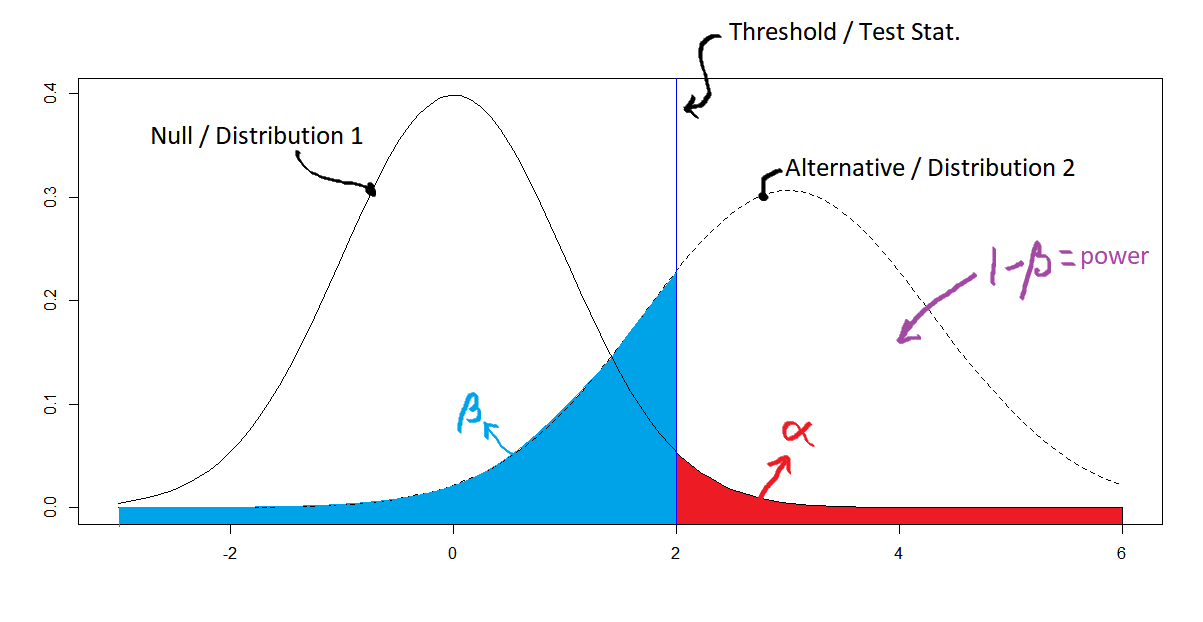
\includegraphics[width=.95\linewidth]{distrsAnno}
			
			Note: \textit{They do NOT need to be normally distributed - they can be normal, uniform, or any other distribution}:
			Most problems will have a decision criteria. They will say, ``Greater than value $ X $ we choose the alternative, else we choose the null''. This $ X $ is the vertical line in the distribution drawn. From here, just think about what each question is asking and how to go about finding the p-values that they are wondering about. 
		}
	
		\mynewcolumn
		
		
		%%%%%%%%%%%%%%%%%%%%%%%%%%%%%%%%%%%%%%%%%%%%%%%%%%%%%%%%%%%%%%%%%%%%%%%%%%%%%%%%
		%                                                                              %
		%                              Linear Regression                               %
		%                                                                              %
		%%%%%%%%%%%%%%%%%%%%%%%%%%%%%%%%%%%%%%%%%%%%%%%%%%%%%%%%%%%%%%%%%%%%%%%%%%%%%%%%
		
		\topic{Linear Regression}{
			Linear regression is all about finding relationships between a response $ Y $ and a predictor $ X $. 
			
			\begin{tellme}{Assumptions}
				\begin{compactitem}
					\item There is a linear relationship between the population of responses and the population of the predictor 
					\item True Errors are Normally Distributed
					\item True Errors have a constant variance (homoscedasticity)
				\end{compactitem}
			\end{tellme}
			
			\begin{tellme}{QuickFacts}
				\begin{compactdesc}
					\item When we \textbf{extrapolate}, we make a prediction of $y$ for an $x$ that is outside of the range that we fit the data on. Imagine that we are predicting the blood pressure of adult males aged 18-40 using a model. We recruit males aged 18 to 40 and then fit our model, but then we are asked to run this model on a 60 year old male or on a female. These points are outside of our sample, and thus we need to be very careful with predictions from our model. 
					\item[Distribution of Test Statistic] If the test is a two sided test, we can use either the T Test Statistic on the $ b_1 $coefficient or the F Test Statistic at the bottom of the test. If it is one-sided, we have to use the T Test Statistic. The F-statistic is related to the T Test Statistic by: $ F = t^2 $ 
					\item[Common Mistakes]  Always be sure to be on the lookout for questions that are testing that you know that \textit{correlation does not imply causation}. Also, always try to write out the form of the regression equation in words - this tends to help out a lot. It is often better to write $Final = b_0 + b_1\times Exam2$ than $\hat{y} = b_0 + b_1x$ to keep them straight on the exam.
				\end{compactdesc}
			\end{tellme}
			
			\begin{tellme}{Interpreting the R Output and Plots}
				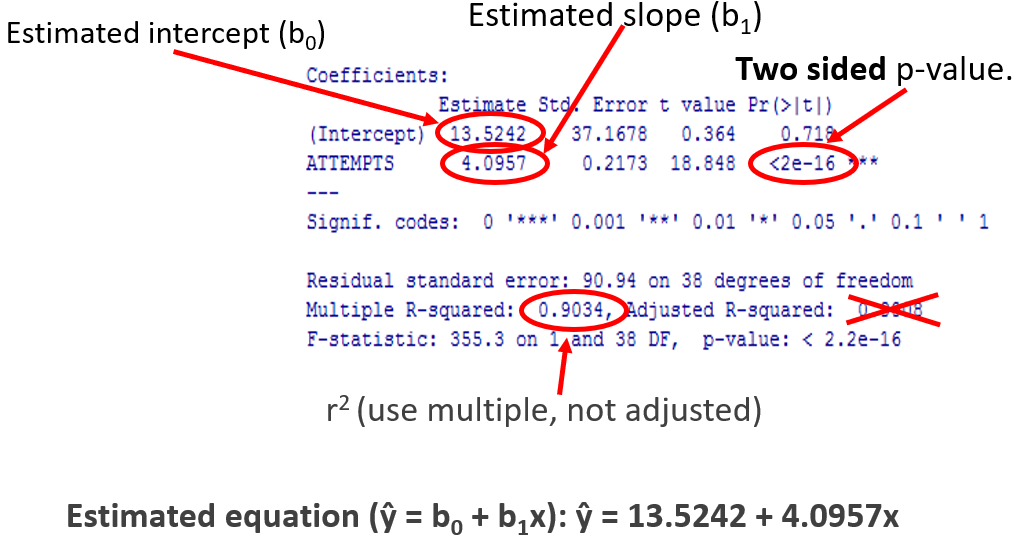
\includegraphics[width=0.95\linewidth]{routput}	
			\end{tellme}
			
			In this class, our interpretation of $ \beta_1 $ is the true change in mean for the response variable for every additional unit increase in the explanatory variable. $R^2$ is the percent of the variation in the response variable explained by the linear relationship between response and predictor 
			
			\begin{compactitem}
				\item A scatter plot can tell us a lot about the relationship between two variables
				\item We can view a scatterplot to look for:
				\begin{compactenum}
					\item Shape/form
					\begin{compactitem}
						\item Linear or non-linear relationship  (does it look like a cup or a rainbow?)
					\end{compactitem}
					\item Direction
					\begin{compactitem}
						\item Positive or negative correlation
					\end{compactitem}
					\item Strength of relationship
					\begin{compactitem}
						\item What's the magnitude of the correlation?
					\end{compactitem}
					\item Potential Outliers
					\begin{compactitem}
						\item Be sure to comment on outliers if you feel there are some
					\end{compactitem}
				\end{compactenum}
				
			\end{compactitem}
		}
		
		%%%%%%%%%%%%%%%%%%%%%%%%%%%%%%%%%%%%%%%%%%%%%%%%%%%%%%%%%%%%%%%%%%%%%%%%%%%%%%%%
		%                                                                              %
		%                                    ANOVA                                     %
		%                                                                              %
		%%%%%%%%%%%%%%%%%%%%%%%%%%%%%%%%%%%%%%%%%%%%%%%%%%%%%%%%%%%%%%%%%%%%%%%%%%%%%%%%
		\mynewcolumn
		
		\topic{ANOVA}{
			Performed when we have $ k $ \textit{independent} populations, and we are trying to test if any of their means differ from one another. This should give you the exact same result as the Tukey test, but it will only provide one p-value instead of each of the pairwise confidence intervals. Note: This test uses an $ F_{k -1, N - k} $ distribution, whereas the Tukey test does not (it uses a special distribution similar to a t-distribution). Always remember the \textsc{Golden Rule}: \textit{Add Down $\rightarrow$ Divide Across} 
			
			\begin{tellme}{Hypothesis \& Assumptions}
				\begin{compactitem}
					\item $ H_0: \mu_1 = \mu_2 = \cdots = \mu_k $
					\item $ H_a: \text{at least one of the $ \mu_i $ is different from the others}$
					\item Each sample is independent of one another
					\item Each \textit{population} is normally distributed (check with $ k $ QQplots)
					\item All population variances have to be equal
				\end{compactitem}
			\end{tellme}
			
			\begin{tellme}{QuickFacts}
				\begin{compactdesc}
					\item[Distribution of Test Statistic] \begin{flushleft}
						$ F_{k -1, N - k} $ Remember - there are two separate degrees of freedom!
					\end{flushleft} \vspace{-8pt} $$F=\frac{\text{Variation among sample means}}{\text{Variation within groups}}=\frac{\text{MS Groups}}{\text{MSE}}$$
					\noindent If the null hypothesis is true, then we expect an F-statistic of approximately one. 
					The larger the $ F $-statistic, the more evidence we have against the hypothesis that all of the means are zero.
					\item[Common Mistakes] Not checking the variance is equal, not remembering the relationships between $ MSE $ and the standard deviation of the population $ s_p $, table manipulation errors (make sure you know how to compute the table! - see example below). 
				\end{compactdesc}
			\end{tellme}
			
			% Plot the F - distribution
			% Created by tikzDevice version 0.10.1 on 2017-11-30 01:12:31
% !TEX encoding = UTF-8 Unicode
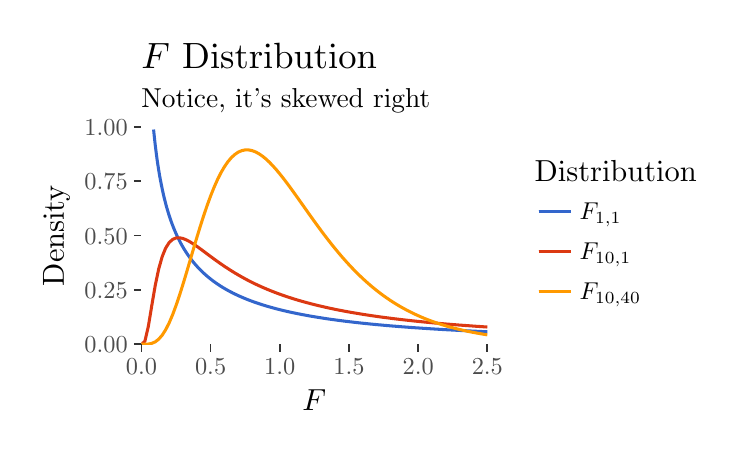
\begin{tikzpicture}[x=1pt,y=1pt]
\definecolor{fillColor}{RGB}{255,255,255}
\path[use as bounding box,fill=fillColor,fill opacity=0.00] (0,0) rectangle (252.94,144.54);
\begin{scope}
\path[clip] ( 41.11, 30.14) rectangle (166.09,108.66);
\definecolor{drawColor}{RGB}{51,102,204}

\path[draw=drawColor,line width= 1.1pt,line join=round] ( 45.50,107.73) --
	( 45.81,104.67) --
	( 46.12,101.89) --
	( 46.44, 99.35) --
	( 46.75, 97.02) --
	( 47.06, 94.88) --
	( 47.38, 92.89) --
	( 47.69, 91.03) --
	( 48.00, 89.31) --
	( 48.32, 87.69) --
	( 48.63, 86.17) --
	( 48.94, 84.74) --
	( 49.25, 83.39) --
	( 49.57, 82.12) --
	( 49.88, 80.91) --
	( 50.19, 79.76) --
	( 50.51, 78.67) --
	( 50.82, 77.63) --
	( 51.13, 76.64) --
	( 51.45, 75.69) --
	( 51.76, 74.78) --
	( 52.07, 73.92) --
	( 52.39, 73.08) --
	( 52.70, 72.28) --
	( 53.01, 71.51) --
	( 53.33, 70.78) --
	( 53.64, 70.06) --
	( 53.95, 69.38) --
	( 54.27, 68.71) --
	( 54.58, 68.08) --
	( 54.89, 67.46) --
	( 55.21, 66.86) --
	( 55.52, 66.28) --
	( 55.83, 65.72) --
	( 56.15, 65.18) --
	( 56.46, 64.65) --
	( 56.77, 64.15) --
	( 57.09, 63.65) --
	( 57.40, 63.17) --
	( 57.71, 62.70) --
	( 58.03, 62.25) --
	( 58.34, 61.81) --
	( 58.65, 61.38) --
	( 58.97, 60.96) --
	( 59.28, 60.55) --
	( 59.59, 60.16) --
	( 59.90, 59.77) --
	( 60.22, 59.39) --
	( 60.53, 59.02) --
	( 60.84, 58.67) --
	( 61.16, 58.32) --
	( 61.47, 57.97) --
	( 61.78, 57.64) --
	( 62.10, 57.31) --
	( 62.41, 56.99) --
	( 62.72, 56.68) --
	( 63.04, 56.38) --
	( 63.35, 56.08) --
	( 63.66, 55.79) --
	( 63.98, 55.50) --
	( 64.29, 55.22) --
	( 64.60, 54.95) --
	( 64.92, 54.68) --
	( 65.23, 54.42) --
	( 65.54, 54.16) --
	( 65.86, 53.91) --
	( 66.17, 53.66) --
	( 66.48, 53.42) --
	( 66.80, 53.18) --
	( 67.11, 52.94) --
	( 67.42, 52.71) --
	( 67.74, 52.49) --
	( 68.05, 52.27) --
	( 68.36, 52.05) --
	( 68.68, 51.84) --
	( 68.99, 51.63) --
	( 69.30, 51.42) --
	( 69.61, 51.22) --
	( 69.93, 51.02) --
	( 70.24, 50.83) --
	( 70.55, 50.64) --
	( 70.87, 50.45) --
	( 71.18, 50.27) --
	( 71.49, 50.08) --
	( 71.81, 49.90) --
	( 72.12, 49.73) --
	( 72.43, 49.55) --
	( 72.75, 49.38) --
	( 73.06, 49.22) --
	( 73.37, 49.05) --
	( 73.69, 48.89) --
	( 74.00, 48.73) --
	( 74.31, 48.57) --
	( 74.63, 48.42) --
	( 74.94, 48.26) --
	( 75.25, 48.11) --
	( 75.57, 47.96) --
	( 75.88, 47.82) --
	( 76.19, 47.68) --
	( 76.51, 47.53) --
	( 76.82, 47.39) --
	( 77.13, 47.26) --
	( 77.45, 47.12) --
	( 77.76, 46.99) --
	( 78.07, 46.85) --
	( 78.39, 46.72) --
	( 78.70, 46.60) --
	( 79.01, 46.47) --
	( 79.33, 46.34) --
	( 79.64, 46.22) --
	( 79.95, 46.10) --
	( 80.26, 45.98) --
	( 80.58, 45.86) --
	( 80.89, 45.75) --
	( 81.20, 45.63) --
	( 81.52, 45.52) --
	( 81.83, 45.40) --
	( 82.14, 45.29) --
	( 82.46, 45.18) --
	( 82.77, 45.08) --
	( 83.08, 44.97) --
	( 83.40, 44.87) --
	( 83.71, 44.76) --
	( 84.02, 44.66) --
	( 84.34, 44.56) --
	( 84.65, 44.46) --
	( 84.96, 44.36) --
	( 85.28, 44.26) --
	( 85.59, 44.16) --
	( 85.90, 44.07) --
	( 86.22, 43.97) --
	( 86.53, 43.88) --
	( 86.84, 43.79) --
	( 87.16, 43.70) --
	( 87.47, 43.61) --
	( 87.78, 43.52) --
	( 88.10, 43.43) --
	( 88.41, 43.35) --
	( 88.72, 43.26) --
	( 89.04, 43.18) --
	( 89.35, 43.09) --
	( 89.66, 43.01) --
	( 89.98, 42.93) --
	( 90.29, 42.85) --
	( 90.60, 42.77) --
	( 90.91, 42.69) --
	( 91.23, 42.61) --
	( 91.54, 42.53) --
	( 91.85, 42.45) --
	( 92.17, 42.38) --
	( 92.48, 42.30) --
	( 92.79, 42.23) --
	( 93.11, 42.16) --
	( 93.42, 42.08) --
	( 93.73, 42.01) --
	( 94.05, 41.94) --
	( 94.36, 41.87) --
	( 94.67, 41.80) --
	( 94.99, 41.73) --
	( 95.30, 41.66) --
	( 95.61, 41.59) --
	( 95.93, 41.53) --
	( 96.24, 41.46) --
	( 96.55, 41.40) --
	( 96.87, 41.33) --
	( 97.18, 41.27) --
	( 97.49, 41.20) --
	( 97.81, 41.14) --
	( 98.12, 41.08) --
	( 98.43, 41.02) --
	( 98.75, 40.95) --
	( 99.06, 40.89) --
	( 99.37, 40.83) --
	( 99.69, 40.77) --
	(100.00, 40.72) --
	(100.31, 40.66) --
	(100.63, 40.60) --
	(100.94, 40.54) --
	(101.25, 40.49) --
	(101.56, 40.43) --
	(101.88, 40.37) --
	(102.19, 40.32) --
	(102.50, 40.27) --
	(102.82, 40.21) --
	(103.13, 40.16) --
	(103.44, 40.10) --
	(103.76, 40.05) --
	(104.07, 40.00) --
	(104.38, 39.95) --
	(104.70, 39.90) --
	(105.01, 39.85) --
	(105.32, 39.80) --
	(105.64, 39.75) --
	(105.95, 39.70) --
	(106.26, 39.65) --
	(106.58, 39.60) --
	(106.89, 39.55) --
	(107.20, 39.50) --
	(107.52, 39.46) --
	(107.83, 39.41) --
	(108.14, 39.36) --
	(108.46, 39.32) --
	(108.77, 39.27) --
	(109.08, 39.23) --
	(109.40, 39.18) --
	(109.71, 39.14) --
	(110.02, 39.09) --
	(110.34, 39.05) --
	(110.65, 39.01) --
	(110.96, 38.96) --
	(111.28, 38.92) --
	(111.59, 38.88) --
	(111.90, 38.84) --
	(112.21, 38.79) --
	(112.53, 38.75) --
	(112.84, 38.71) --
	(113.15, 38.67) --
	(113.47, 38.63) --
	(113.78, 38.59) --
	(114.09, 38.55) --
	(114.41, 38.51) --
	(114.72, 38.47) --
	(115.03, 38.43) --
	(115.35, 38.40) --
	(115.66, 38.36) --
	(115.97, 38.32) --
	(116.29, 38.28) --
	(116.60, 38.25) --
	(116.91, 38.21) --
	(117.23, 38.17) --
	(117.54, 38.14) --
	(117.85, 38.10) --
	(118.17, 38.06) --
	(118.48, 38.03) --
	(118.79, 37.99) --
	(119.11, 37.96) --
	(119.42, 37.92) --
	(119.73, 37.89) --
	(120.05, 37.86) --
	(120.36, 37.82) --
	(120.67, 37.79) --
	(120.99, 37.75) --
	(121.30, 37.72) --
	(121.61, 37.69) --
	(121.93, 37.66) --
	(122.24, 37.62) --
	(122.55, 37.59) --
	(122.86, 37.56) --
	(123.18, 37.53) --
	(123.49, 37.50) --
	(123.80, 37.46) --
	(124.12, 37.43) --
	(124.43, 37.40) --
	(124.74, 37.37) --
	(125.06, 37.34) --
	(125.37, 37.31) --
	(125.68, 37.28) --
	(126.00, 37.25) --
	(126.31, 37.22) --
	(126.62, 37.19) --
	(126.94, 37.16) --
	(127.25, 37.13) --
	(127.56, 37.11) --
	(127.88, 37.08) --
	(128.19, 37.05) --
	(128.50, 37.02) --
	(128.82, 36.99) --
	(129.13, 36.97) --
	(129.44, 36.94) --
	(129.76, 36.91) --
	(130.07, 36.88) --
	(130.38, 36.86) --
	(130.70, 36.83) --
	(131.01, 36.80) --
	(131.32, 36.78) --
	(131.64, 36.75) --
	(131.95, 36.72) --
	(132.26, 36.70) --
	(132.58, 36.67) --
	(132.89, 36.65) --
	(133.20, 36.62) --
	(133.51, 36.60) --
	(133.83, 36.57) --
	(134.14, 36.55) --
	(134.45, 36.52) --
	(134.77, 36.50) --
	(135.08, 36.47) --
	(135.39, 36.45) --
	(135.71, 36.42) --
	(136.02, 36.40) --
	(136.33, 36.38) --
	(136.65, 36.35) --
	(136.96, 36.33) --
	(137.27, 36.31) --
	(137.59, 36.28) --
	(137.90, 36.26) --
	(138.21, 36.24) --
	(138.53, 36.21) --
	(138.84, 36.19) --
	(139.15, 36.17) --
	(139.47, 36.15) --
	(139.78, 36.13) --
	(140.09, 36.10) --
	(140.41, 36.08) --
	(140.72, 36.06) --
	(141.03, 36.04) --
	(141.35, 36.02) --
	(141.66, 35.99) --
	(141.97, 35.97) --
	(142.29, 35.95) --
	(142.60, 35.93) --
	(142.91, 35.91) --
	(143.23, 35.89) --
	(143.54, 35.87) --
	(143.85, 35.85) --
	(144.16, 35.83) --
	(144.48, 35.81) --
	(144.79, 35.79) --
	(145.10, 35.77) --
	(145.42, 35.75) --
	(145.73, 35.73) --
	(146.04, 35.71) --
	(146.36, 35.69) --
	(146.67, 35.67) --
	(146.98, 35.65) --
	(147.30, 35.63) --
	(147.61, 35.61) --
	(147.92, 35.59) --
	(148.24, 35.57) --
	(148.55, 35.56) --
	(148.86, 35.54) --
	(149.18, 35.52) --
	(149.49, 35.50) --
	(149.80, 35.48) --
	(150.12, 35.46) --
	(150.43, 35.45) --
	(150.74, 35.43) --
	(151.06, 35.41) --
	(151.37, 35.39) --
	(151.68, 35.37) --
	(152.00, 35.36) --
	(152.31, 35.34) --
	(152.62, 35.32) --
	(152.94, 35.31) --
	(153.25, 35.29) --
	(153.56, 35.27) --
	(153.88, 35.25) --
	(154.19, 35.24) --
	(154.50, 35.22) --
	(154.81, 35.20) --
	(155.13, 35.19) --
	(155.44, 35.17) --
	(155.75, 35.15) --
	(156.07, 35.14) --
	(156.38, 35.12) --
	(156.69, 35.11) --
	(157.01, 35.09) --
	(157.32, 35.07) --
	(157.63, 35.06) --
	(157.95, 35.04) --
	(158.26, 35.03) --
	(158.57, 35.01) --
	(158.89, 34.99) --
	(159.20, 34.98) --
	(159.51, 34.96) --
	(159.83, 34.95) --
	(160.14, 34.93) --
	(160.45, 34.92) --
	(160.77, 34.90) --
	(161.08, 34.89) --
	(161.39, 34.87) --
	(161.71, 34.86) --
	(162.02, 34.84) --
	(162.33, 34.83) --
	(162.65, 34.81) --
	(162.96, 34.80) --
	(163.27, 34.79) --
	(163.59, 34.77) --
	(163.90, 34.76) --
	(164.21, 34.74) --
	(164.53, 34.73) --
	(164.84, 34.71) --
	(165.15, 34.70) --
	(165.46, 34.69) --
	(165.78, 34.67) --
	(166.09, 34.66);
\definecolor{drawColor}{RGB}{220,57,18}

\path[draw=drawColor,line width= 1.1pt,line join=round] ( 41.11, 30.14) --
	( 42.36, 31.25) --
	( 43.61, 36.64) --
	( 44.86, 44.22) --
	( 46.11, 51.49) --
	( 47.36, 57.41) --
	( 48.61, 61.82) --
	( 49.86, 64.89) --
	( 51.11, 66.87) --
	( 52.36, 68.02) --
	( 53.61, 68.55) --
	( 54.86, 68.62) --
	( 56.11, 68.36) --
	( 57.36, 67.85) --
	( 58.61, 67.18) --
	( 59.86, 66.40) --
	( 61.11, 65.54) --
	( 62.36, 64.64) --
	( 63.61, 63.71) --
	( 64.86, 62.78) --
	( 66.11, 61.85) --
	( 67.36, 60.93) --
	( 68.61, 60.03) --
	( 69.86, 59.15) --
	( 71.11, 58.30) --
	( 72.36, 57.48) --
	( 73.61, 56.68) --
	( 74.86, 55.91) --
	( 76.11, 55.17) --
	( 77.36, 54.46) --
	( 78.60, 53.77) --
	( 79.85, 53.12) --
	( 81.10, 52.48) --
	( 82.35, 51.87) --
	( 83.60, 51.29) --
	( 84.85, 50.73) --
	( 86.10, 50.19) --
	( 87.35, 49.67) --
	( 88.60, 49.17) --
	( 89.85, 48.69) --
	( 91.10, 48.23) --
	( 92.35, 47.79) --
	( 93.60, 47.36) --
	( 94.85, 46.95) --
	( 96.10, 46.55) --
	( 97.35, 46.17) --
	( 98.60, 45.80) --
	( 99.85, 45.45) --
	(101.10, 45.11) --
	(102.35, 44.78) --
	(103.60, 44.46) --
	(104.85, 44.15) --
	(106.10, 43.86) --
	(107.35, 43.57) --
	(108.60, 43.29) --
	(109.85, 43.02) --
	(111.10, 42.76) --
	(112.35, 42.51) --
	(113.60, 42.27) --
	(114.85, 42.03) --
	(116.10, 41.80) --
	(117.35, 41.58) --
	(118.60, 41.37) --
	(119.85, 41.16) --
	(121.10, 40.96) --
	(122.35, 40.76) --
	(123.60, 40.57) --
	(124.85, 40.39) --
	(126.10, 40.21) --
	(127.35, 40.03) --
	(128.60, 39.86) --
	(129.85, 39.70) --
	(131.10, 39.54) --
	(132.35, 39.38) --
	(133.60, 39.23) --
	(134.85, 39.08) --
	(136.10, 38.94) --
	(137.35, 38.80) --
	(138.60, 38.66) --
	(139.85, 38.53) --
	(141.10, 38.40) --
	(142.34, 38.28) --
	(143.59, 38.15) --
	(144.84, 38.03) --
	(146.09, 37.92) --
	(147.34, 37.80) --
	(148.59, 37.69) --
	(149.84, 37.58) --
	(151.09, 37.47) --
	(152.34, 37.37) --
	(153.59, 37.27) --
	(154.84, 37.17) --
	(156.09, 37.07) --
	(157.34, 36.98) --
	(158.59, 36.89) --
	(159.84, 36.80) --
	(161.09, 36.71) --
	(162.34, 36.62) --
	(163.59, 36.54) --
	(164.84, 36.45) --
	(166.09, 36.37);
\definecolor{drawColor}{RGB}{255,153,0}

\path[draw=drawColor,line width= 1.1pt,line join=round] ( 41.11, 30.14) --
	( 42.36, 30.15) --
	( 43.61, 30.22) --
	( 44.86, 30.47) --
	( 46.11, 31.02) --
	( 47.36, 31.99) --
	( 48.61, 33.43) --
	( 49.86, 35.38) --
	( 51.11, 37.84) --
	( 52.36, 40.78) --
	( 53.61, 44.13) --
	( 54.86, 47.82) --
	( 56.11, 51.79) --
	( 57.36, 55.93) --
	( 58.61, 60.18) --
	( 59.86, 64.44) --
	( 61.11, 68.65) --
	( 62.36, 72.73) --
	( 63.61, 76.64) --
	( 64.86, 80.32) --
	( 66.11, 83.74) --
	( 67.36, 86.87) --
	( 68.61, 89.68) --
	( 69.86, 92.16) --
	( 71.11, 94.30) --
	( 72.36, 96.11) --
	( 73.61, 97.58) --
	( 74.86, 98.73) --
	( 76.11, 99.57) --
	( 77.36,100.11) --
	( 78.60,100.37) --
	( 79.85,100.36) --
	( 81.10,100.11) --
	( 82.35, 99.64) --
	( 83.60, 98.96) --
	( 84.85, 98.10) --
	( 86.10, 97.08) --
	( 87.35, 95.91) --
	( 88.60, 94.61) --
	( 89.85, 93.21) --
	( 91.10, 91.71) --
	( 92.35, 90.13) --
	( 93.60, 88.50) --
	( 94.85, 86.81) --
	( 96.10, 85.08) --
	( 97.35, 83.34) --
	( 98.60, 81.57) --
	( 99.85, 79.80) --
	(101.10, 78.03) --
	(102.35, 76.27) --
	(103.60, 74.53) --
	(104.85, 72.81) --
	(106.10, 71.11) --
	(107.35, 69.45) --
	(108.60, 67.82) --
	(109.85, 66.23) --
	(111.10, 64.68) --
	(112.35, 63.17) --
	(113.60, 61.70) --
	(114.85, 60.28) --
	(116.10, 58.91) --
	(117.35, 57.58) --
	(118.60, 56.30) --
	(119.85, 55.06) --
	(121.10, 53.88) --
	(122.35, 52.73) --
	(123.60, 51.64) --
	(124.85, 50.58) --
	(126.10, 49.57) --
	(127.35, 48.61) --
	(128.60, 47.68) --
	(129.85, 46.80) --
	(131.10, 45.95) --
	(132.35, 45.15) --
	(133.60, 44.38) --
	(134.85, 43.64) --
	(136.10, 42.95) --
	(137.35, 42.28) --
	(138.60, 41.65) --
	(139.85, 41.04) --
	(141.10, 40.47) --
	(142.34, 39.92) --
	(143.59, 39.40) --
	(144.84, 38.91) --
	(146.09, 38.44) --
	(147.34, 38.00) --
	(148.59, 37.58) --
	(149.84, 37.18) --
	(151.09, 36.80) --
	(152.34, 36.44) --
	(153.59, 36.10) --
	(154.84, 35.78) --
	(156.09, 35.48) --
	(157.34, 35.19) --
	(158.59, 34.91) --
	(159.84, 34.65) --
	(161.09, 34.41) --
	(162.34, 34.18) --
	(163.59, 33.96) --
	(164.84, 33.75) --
	(166.09, 33.55);
\end{scope}
\begin{scope}
\path[clip] (  0.00,  0.00) rectangle (252.94,144.54);
\definecolor{drawColor}{gray}{0.30}

\node[text=drawColor,anchor=base east,inner sep=0pt, outer sep=0pt, scale=  0.88] at ( 36.16, 27.11) {0.00};

\node[text=drawColor,anchor=base east,inner sep=0pt, outer sep=0pt, scale=  0.88] at ( 36.16, 46.74) {0.25};

\node[text=drawColor,anchor=base east,inner sep=0pt, outer sep=0pt, scale=  0.88] at ( 36.16, 66.37) {0.50};

\node[text=drawColor,anchor=base east,inner sep=0pt, outer sep=0pt, scale=  0.88] at ( 36.16, 86.00) {0.75};

\node[text=drawColor,anchor=base east,inner sep=0pt, outer sep=0pt, scale=  0.88] at ( 36.16,105.63) {1.00};
\end{scope}
\begin{scope}
\path[clip] (  0.00,  0.00) rectangle (252.94,144.54);
\definecolor{drawColor}{gray}{0.20}

\path[draw=drawColor,line width= 0.6pt,line join=round] ( 38.36, 30.14) --
	( 41.11, 30.14);

\path[draw=drawColor,line width= 0.6pt,line join=round] ( 38.36, 49.77) --
	( 41.11, 49.77);

\path[draw=drawColor,line width= 0.6pt,line join=round] ( 38.36, 69.40) --
	( 41.11, 69.40);

\path[draw=drawColor,line width= 0.6pt,line join=round] ( 38.36, 89.03) --
	( 41.11, 89.03);

\path[draw=drawColor,line width= 0.6pt,line join=round] ( 38.36,108.66) --
	( 41.11,108.66);
\end{scope}
\begin{scope}
\path[clip] (  0.00,  0.00) rectangle (252.94,144.54);
\definecolor{drawColor}{gray}{0.20}

\path[draw=drawColor,line width= 0.6pt,line join=round] ( 41.11, 27.39) --
	( 41.11, 30.14);

\path[draw=drawColor,line width= 0.6pt,line join=round] ( 66.11, 27.39) --
	( 66.11, 30.14);

\path[draw=drawColor,line width= 0.6pt,line join=round] ( 91.10, 27.39) --
	( 91.10, 30.14);

\path[draw=drawColor,line width= 0.6pt,line join=round] (116.10, 27.39) --
	(116.10, 30.14);

\path[draw=drawColor,line width= 0.6pt,line join=round] (141.10, 27.39) --
	(141.10, 30.14);

\path[draw=drawColor,line width= 0.6pt,line join=round] (166.09, 27.39) --
	(166.09, 30.14);
\end{scope}
\begin{scope}
\path[clip] (  0.00,  0.00) rectangle (252.94,144.54);
\definecolor{drawColor}{gray}{0.30}

\node[text=drawColor,anchor=base,inner sep=0pt, outer sep=0pt, scale=  0.88] at ( 41.11, 19.13) {0.0};

\node[text=drawColor,anchor=base,inner sep=0pt, outer sep=0pt, scale=  0.88] at ( 66.11, 19.13) {0.5};

\node[text=drawColor,anchor=base,inner sep=0pt, outer sep=0pt, scale=  0.88] at ( 91.10, 19.13) {1.0};

\node[text=drawColor,anchor=base,inner sep=0pt, outer sep=0pt, scale=  0.88] at (116.10, 19.13) {1.5};

\node[text=drawColor,anchor=base,inner sep=0pt, outer sep=0pt, scale=  0.88] at (141.10, 19.13) {2.0};

\node[text=drawColor,anchor=base,inner sep=0pt, outer sep=0pt, scale=  0.88] at (166.09, 19.13) {2.5};
\end{scope}
\begin{scope}
\path[clip] (  0.00,  0.00) rectangle (252.94,144.54);
\definecolor{drawColor}{RGB}{0,0,0}

\node[text=drawColor,anchor=base,inner sep=0pt, outer sep=0pt, scale=  1.10] at (103.60,  6.06) {$F$};
\end{scope}
\begin{scope}
\path[clip] (  0.00,  0.00) rectangle (252.94,144.54);
\definecolor{drawColor}{RGB}{0,0,0}

\node[text=drawColor,rotate= 90.00,anchor=base,inner sep=0pt, outer sep=0pt, scale=  1.10] at ( 13.08, 69.40) {Density};
\end{scope}
\begin{scope}
\path[clip] (  0.00,  0.00) rectangle (252.94,144.54);
\definecolor{drawColor}{RGB}{0,0,0}

\node[text=drawColor,anchor=base west,inner sep=0pt, outer sep=0pt, scale=  1.10] at (183.16, 89.10) {Distribution};
\end{scope}
\begin{scope}
\path[clip] (  0.00,  0.00) rectangle (252.94,144.54);
\definecolor{drawColor}{RGB}{51,102,204}

\path[draw=drawColor,line width= 1.1pt,line join=round] (184.61, 78.26) -- (196.17, 78.26);
\end{scope}
\begin{scope}
\path[clip] (  0.00,  0.00) rectangle (252.94,144.54);
\definecolor{drawColor}{RGB}{51,102,204}

\path[draw=drawColor,line width= 1.1pt,line join=round] (184.61, 78.26) -- (196.17, 78.26);
\end{scope}
\begin{scope}
\path[clip] (  0.00,  0.00) rectangle (252.94,144.54);
\definecolor{drawColor}{RGB}{51,102,204}

\path[draw=drawColor,line width= 1.1pt,line join=round] (184.61, 78.26) -- (196.17, 78.26);
\end{scope}
\begin{scope}
\path[clip] (  0.00,  0.00) rectangle (252.94,144.54);
\definecolor{drawColor}{RGB}{220,57,18}

\path[draw=drawColor,line width= 1.1pt,line join=round] (184.61, 63.81) -- (196.17, 63.81);
\end{scope}
\begin{scope}
\path[clip] (  0.00,  0.00) rectangle (252.94,144.54);
\definecolor{drawColor}{RGB}{220,57,18}

\path[draw=drawColor,line width= 1.1pt,line join=round] (184.61, 63.81) -- (196.17, 63.81);
\end{scope}
\begin{scope}
\path[clip] (  0.00,  0.00) rectangle (252.94,144.54);
\definecolor{drawColor}{RGB}{220,57,18}

\path[draw=drawColor,line width= 1.1pt,line join=round] (184.61, 63.81) -- (196.17, 63.81);
\end{scope}
\begin{scope}
\path[clip] (  0.00,  0.00) rectangle (252.94,144.54);
\definecolor{drawColor}{RGB}{255,153,0}

\path[draw=drawColor,line width= 1.1pt,line join=round] (184.61, 49.35) -- (196.17, 49.35);
\end{scope}
\begin{scope}
\path[clip] (  0.00,  0.00) rectangle (252.94,144.54);
\definecolor{drawColor}{RGB}{255,153,0}

\path[draw=drawColor,line width= 1.1pt,line join=round] (184.61, 49.35) -- (196.17, 49.35);
\end{scope}
\begin{scope}
\path[clip] (  0.00,  0.00) rectangle (252.94,144.54);
\definecolor{drawColor}{RGB}{255,153,0}

\path[draw=drawColor,line width= 1.1pt,line join=round] (184.61, 49.35) -- (196.17, 49.35);
\end{scope}
\begin{scope}
\path[clip] (  0.00,  0.00) rectangle (252.94,144.54);
\definecolor{drawColor}{RGB}{0,0,0}

\node[text=drawColor,anchor=base west,inner sep=0pt, outer sep=0pt, scale=  0.88] at (199.42, 75.23) {$F_{1,1}$};
\end{scope}
\begin{scope}
\path[clip] (  0.00,  0.00) rectangle (252.94,144.54);
\definecolor{drawColor}{RGB}{0,0,0}

\node[text=drawColor,anchor=base west,inner sep=0pt, outer sep=0pt, scale=  0.88] at (199.42, 60.78) {$F_{10,1}$};
\end{scope}
\begin{scope}
\path[clip] (  0.00,  0.00) rectangle (252.94,144.54);
\definecolor{drawColor}{RGB}{0,0,0}

\node[text=drawColor,anchor=base west,inner sep=0pt, outer sep=0pt, scale=  0.88] at (199.42, 46.32) {$F_{10,40}$};
\end{scope}
\begin{scope}
\path[clip] (  0.00,  0.00) rectangle (252.94,144.54);
\definecolor{drawColor}{RGB}{0,0,0}

\node[text=drawColor,anchor=base west,inner sep=0pt, outer sep=0pt, scale=  0.99] at ( 41.11,115.56) {Notice, it's skewed right};
\end{scope}
\begin{scope}
\path[clip] (  0.00,  0.00) rectangle (252.94,144.54);
\definecolor{drawColor}{RGB}{0,0,0}

\node[text=drawColor,anchor=base west,inner sep=0pt, outer sep=0pt, scale=  1.32] at ( 41.11,129.95) {$F$ Distribution};
\end{scope}
\end{tikzpicture}

			
			\begin{tellme}{Example}
				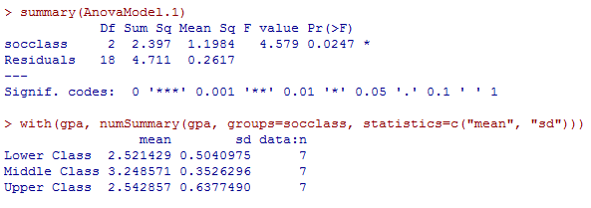
\includegraphics[width=\linewidth]{anova_output}
				\begin{compactitem}
					\item MSE is 0.2617
					\item MS Groups is 1.1984
					\item $F=\frac{1.1984}{0.2617}=4.579$
					\item $d_1=k-1=3-1=2$
					\item $d_2=N-k=N-3=18$
					\item P-value is 0.0247
				\end{compactitem}
			\end{tellme}
			\vspace{1cm}
			\begin{tellme}{Example}
				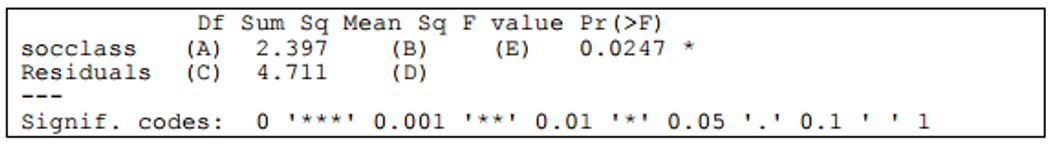
\includegraphics[width=\linewidth]{cool_down}
				\begin{compactenum}
					\item We know there are $k=3$ groups, so the numerator degrees of freedom (A) must be: 2
					\item We divide SS Groups: 2.397 by the numerator df (A) 2 to obtain the MS Groups (B): 1.1984
					\item We know there are $N=21$ total observations, so the denominator df (C) must be: $N-k=18$
					\item We divide the SS Error by the denominator df (C) to obtain the MS Error (D) of: 0.2617
					\item We divide the MS Groups (B): 1.1984 by the MS Error (D) 0.2617 to get the $ F $ statistic: 4.57
				\end{compactenum} 
			\end{tellme}
		}
		%%%%%%%%%%%%%%%%%%%%%%%%%%%%%%%%%%%%%%%%%%%%%%%%%%%%%%%%%%%%%%%%%%%%%%%%%%%%%%%%
		%                                                                              %
		%                                 Chi Squared                                  %
		%                                                                              %
		%%%%%%%%%%%%%%%%%%%%%%%%%%%%%%%%%%%%%%%%%%%%%%%%%%%%%%%%%%%%%%%%%%%%%%%%%%%%%%%%
		
		\topic{Chi-Squared}{
			There are three different types of Chi-Squared tests. 
			\begin{compactitem}
				\item Test of Independence
				\item Test of Homogeneity
				\item Goodness of Fit
			\end{compactitem}
			Each test uses the same test statistic given by: 
			\begin{align*}
			\chi^{2} = \sum\limits_{i = 1}^{n} \frac{(\text{Observed} - \text{Expected})^{2}}{\text{Expected}} \,\, {\bigg \vert} \,\, \text{Contribution} = \frac{(\text{Obs} - \text{Exp})^{2}}{\text{Exp}} 
			\end{align*}
			The further away our observation is away from what we would expect, the larger the test statistic.
			
			\begin{tellme}{Discerning the Three Types of Tests}
				\begin{compactdesc}
					\item[Goodness of Fit]  
					This test answers the question, ``Do the data fit well compared to a specified distribution?'' It considers one categorical response, and assesses whether the proportion of sampled observations falling into each category matches well to a specified distribution. The null hypothesis specifies this distribution which describes the population proportion of observations in each category.
					%	There is one population and one categorical variable.
					Ex: Imagine that one grabs a bag of MM's. MM's lists the color distribution as: According to it, each package of Milk Chocolate M\&M’s should contain 24\% blue, 14\% brown, 16\% green, 20\% orange, 13\% red, and 14\% yellow M\&M’s. We could take a few packs of MM's and compare our observed percentages to what we would expect to see if we are getting results consistent with MM's website. 
					
					\item[Test of Homogeneity] 
					This test answers the question, ``Do two or more populations have the same distribution for one categorical variable?''  It considers one categorical response, and assesses whether the model for this response is the same in two (or more) populations. The null hypothesis is that the distribution of the categorical variable is the same for the two (or more) populations.
					%	We have one categorical variable and two or more populations.
					Ex. I have five TV shows and I am trying to see if each of the proportions of men and women are the same across the five shows. 
					
					\item[Test of Independence] This test answers the question, ``Are two factors (or variables) independent for a population under study?'' It considers two categorical variables (sometimes one is a response and the other is explanatory), and assesses whether there appears to be a relationship between these two variables for a single population. The null hypothesis is that the two categorical variables are independent (not related) for the population of interest. 
					%	We have two categorical variables and one population. 
					Ex: Imagine that I was trying to determine if someones school year (Freshman, Sophomore, Junior, Senior), is independent of where they live on campus (in the dorms, off campus, at home, fraternity / sorority) 
				\end{compactdesc}
			\end{tellme}
			
			\begin{tellme}{Variables and Populations}
				\begin{center}
					\begin{tabular}{ccc}
						\toprule
						\textbf{Test} & \textbf{Number of Variables} & \textbf{Number of Populations} \\ 
						\midrule
						Goodness of Fit & 1 & 1 \\ 
						Homogeneity & 1 & 2+ \\ 
						Independence & 2 & 1\\
						\bottomrule
					\end{tabular} 
				\end{center}
			\end{tellme}
			
			\vspace{4mm}
			\newcommand{\varfil}[1]{\ensuremath{\langle #1 \rangle}\xspace}
			\begin{tellme}{Null Hypothesis}
				\begin{compactdesc}
					\item[Goodness of Fit] \begin{flushleft}
						$ H_0: $ $ p_1 = \varfil{PopulationProp_1} $, $ p_2 = \varfil{PopulationProp_2} $, \ldots, $ p_k = \varfil{PopulationProp_k} $.
					\end{flushleft}
					\item[Homogeneity] $ H_0: $ The distribution of \varfil{VariableNames} is the same for populations of \varfil{Names of the Populations}
					\item[Independence] $ H_0: $ There is no relationship between \varfil{Variable1} and \varfil{Variable2}
				\end{compactdesc}
			\end{tellme}
			
			\begin{tellme}{Independence vs. Homogeneity}
				You'll see that the test for independence and homogeneity are easily confused. Some quick tips:
				\begin{compactitem}
					\item Check the sampling method and the problem setup
					\item In tests for Homogeneity, we have two or more populations and only one variable. In independence testing we have one population and more than one variable.
					\item In tests for Homogeneity, we have two or more samples. In independence tests, we have one sample and record two variables
					\item In tests for Homogeneity, the question is asking if the populations are \textit{different}. In tests for independence, we are asking if the \textit{variables} are \textit{independent} or \textit{associated}
					\item What if...
					\begin{compactitem}
						\item I took a random sample of wedding guests and recorded if they were from the bride’s side or the groom’s side and what type of meal they wanted. (Independence)
						\item I took a random sample of wedding guests from the bride’s side and a second random sample from the groom’s side and recorded what type of meal they wanted. (Homogeneity)
					\end{compactitem}
				\end{compactitem}
			\end{tellme}
			
			\begin{tellme}{The Chi-Squared Distribution}
				
				% Created by tikzDevice version 0.10.1 on 2017-12-04 18:39:09
% !TEX encoding = UTF-8 Unicode
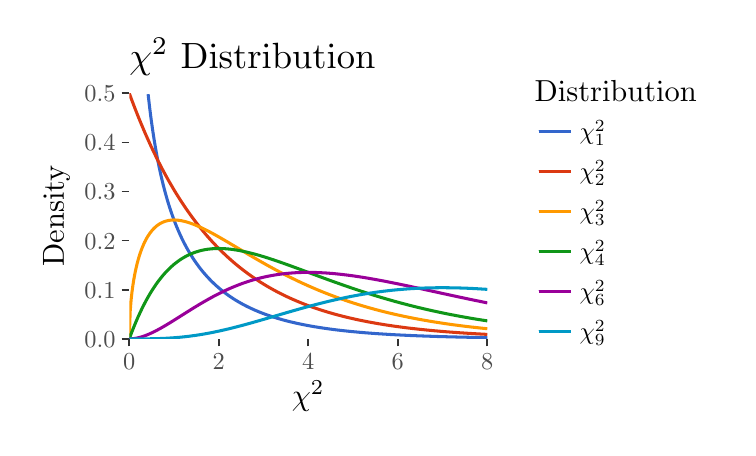
\begin{tikzpicture}[x=1pt,y=1pt]
\definecolor{fillColor}{RGB}{255,255,255}
\path[use as bounding box,fill=fillColor,fill opacity=0.00] (0,0) rectangle (252.94,144.54);
\begin{scope}
\path[clip] ( 36.71, 32.09) rectangle (166.09,120.85);
\definecolor{drawColor}{RGB}{51,102,204}

\path[draw=drawColor,line width= 1.1pt,line join=round] ( 43.52,120.51) --
	( 43.85,117.62) --
	( 44.17,114.90) --
	( 44.49,112.35) --
	( 44.82,109.94) --
	( 45.14,107.67) --
	( 45.47,105.52) --
	( 45.79,103.47) --
	( 46.12,101.53) --
	( 46.44, 99.69) --
	( 46.76, 97.92) --
	( 47.09, 96.24) --
	( 47.41, 94.63) --
	( 47.74, 93.09) --
	( 48.06, 91.61) --
	( 48.39, 90.19) --
	( 48.71, 88.83) --
	( 49.03, 87.52) --
	( 49.36, 86.26) --
	( 49.68, 85.04) --
	( 50.01, 83.87) --
	( 50.33, 82.74) --
	( 50.65, 81.65) --
	( 50.98, 80.59) --
	( 51.30, 79.57) --
	( 51.63, 78.59) --
	( 51.95, 77.63) --
	( 52.28, 76.70) --
	( 52.60, 75.81) --
	( 52.92, 74.93) --
	( 53.25, 74.09) --
	( 53.57, 73.27) --
	( 53.90, 72.47) --
	( 54.22, 71.70) --
	( 54.55, 70.94) --
	( 54.87, 70.21) --
	( 55.19, 69.50) --
	( 55.52, 68.80) --
	( 55.84, 68.13) --
	( 56.17, 67.47) --
	( 56.49, 66.83) --
	( 56.82, 66.20) --
	( 57.14, 65.59) --
	( 57.46, 65.00) --
	( 57.79, 64.42) --
	( 58.11, 63.85) --
	( 58.44, 63.30) --
	( 58.76, 62.76) --
	( 59.09, 62.24) --
	( 59.41, 61.72) --
	( 59.73, 61.22) --
	( 60.06, 60.73) --
	( 60.38, 60.25) --
	( 60.71, 59.78) --
	( 61.03, 59.32) --
	( 61.36, 58.87) --
	( 61.68, 58.43) --
	( 62.00, 58.00) --
	( 62.33, 57.57) --
	( 62.65, 57.16) --
	( 62.98, 56.76) --
	( 63.30, 56.36) --
	( 63.63, 55.98) --
	( 63.95, 55.60) --
	( 64.27, 55.22) --
	( 64.60, 54.86) --
	( 64.92, 54.50) --
	( 65.25, 54.15) --
	( 65.57, 53.81) --
	( 65.90, 53.47) --
	( 66.22, 53.14) --
	( 66.54, 52.82) --
	( 66.87, 52.50) --
	( 67.19, 52.19) --
	( 67.52, 51.88) --
	( 67.84, 51.59) --
	( 68.16, 51.29) --
	( 68.49, 51.00) --
	( 68.81, 50.72) --
	( 69.14, 50.44) --
	( 69.46, 50.17) --
	( 69.79, 49.90) --
	( 70.11, 49.64) --
	( 70.43, 49.38) --
	( 70.76, 49.12) --
	( 71.08, 48.87) --
	( 71.41, 48.63) --
	( 71.73, 48.39) --
	( 72.06, 48.15) --
	( 72.38, 47.92) --
	( 72.70, 47.69) --
	( 73.03, 47.46) --
	( 73.35, 47.24) --
	( 73.68, 47.03) --
	( 74.00, 46.81) --
	( 74.33, 46.60) --
	( 74.65, 46.40) --
	( 74.97, 46.19) --
	( 75.30, 45.99) --
	( 75.62, 45.80) --
	( 75.95, 45.60) --
	( 76.27, 45.41) --
	( 76.60, 45.23) --
	( 76.92, 45.04) --
	( 77.24, 44.86) --
	( 77.57, 44.69) --
	( 77.89, 44.51) --
	( 78.22, 44.34) --
	( 78.54, 44.17) --
	( 78.87, 44.00) --
	( 79.19, 43.84) --
	( 79.51, 43.68) --
	( 79.84, 43.52) --
	( 80.16, 43.36) --
	( 80.49, 43.21) --
	( 80.81, 43.06) --
	( 81.14, 42.91) --
	( 81.46, 42.76) --
	( 81.78, 42.62) --
	( 82.11, 42.47) --
	( 82.43, 42.33) --
	( 82.76, 42.20) --
	( 83.08, 42.06) --
	( 83.41, 41.93) --
	( 83.73, 41.79) --
	( 84.05, 41.66) --
	( 84.38, 41.54) --
	( 84.70, 41.41) --
	( 85.03, 41.29) --
	( 85.35, 41.16) --
	( 85.67, 41.04) --
	( 86.00, 40.93) --
	( 86.32, 40.81) --
	( 86.65, 40.69) --
	( 86.97, 40.58) --
	( 87.30, 40.47) --
	( 87.62, 40.36) --
	( 87.94, 40.25) --
	( 88.27, 40.14) --
	( 88.59, 40.04) --
	( 88.92, 39.93) --
	( 89.24, 39.83) --
	( 89.57, 39.73) --
	( 89.89, 39.63) --
	( 90.21, 39.53) --
	( 90.54, 39.44) --
	( 90.86, 39.34) --
	( 91.19, 39.25) --
	( 91.51, 39.16) --
	( 91.84, 39.06) --
	( 92.16, 38.97) --
	( 92.48, 38.89) --
	( 92.81, 38.80) --
	( 93.13, 38.71) --
	( 93.46, 38.63) --
	( 93.78, 38.54) --
	( 94.11, 38.46) --
	( 94.43, 38.38) --
	( 94.75, 38.30) --
	( 95.08, 38.22) --
	( 95.40, 38.14) --
	( 95.73, 38.07) --
	( 96.05, 37.99) --
	( 96.38, 37.92) --
	( 96.70, 37.84) --
	( 97.02, 37.77) --
	( 97.35, 37.70) --
	( 97.67, 37.63) --
	( 98.00, 37.56) --
	( 98.32, 37.49) --
	( 98.65, 37.42) --
	( 98.97, 37.35) --
	( 99.29, 37.29) --
	( 99.62, 37.22) --
	( 99.94, 37.16) --
	(100.27, 37.09) --
	(100.59, 37.03) --
	(100.92, 36.97) --
	(101.24, 36.91) --
	(101.56, 36.85) --
	(101.89, 36.79) --
	(102.21, 36.73) --
	(102.54, 36.67) --
	(102.86, 36.62) --
	(103.18, 36.56) --
	(103.51, 36.50) --
	(103.83, 36.45) --
	(104.16, 36.40) --
	(104.48, 36.34) --
	(104.81, 36.29) --
	(105.13, 36.24) --
	(105.45, 36.19) --
	(105.78, 36.14) --
	(106.10, 36.09) --
	(106.43, 36.04) --
	(106.75, 35.99) --
	(107.08, 35.94) --
	(107.40, 35.89) --
	(107.72, 35.85) --
	(108.05, 35.80) --
	(108.37, 35.76) --
	(108.70, 35.71) --
	(109.02, 35.67) --
	(109.35, 35.62) --
	(109.67, 35.58) --
	(109.99, 35.54) --
	(110.32, 35.50) --
	(110.64, 35.45) --
	(110.97, 35.41) --
	(111.29, 35.37) --
	(111.62, 35.33) --
	(111.94, 35.29) --
	(112.26, 35.26) --
	(112.59, 35.22) --
	(112.91, 35.18) --
	(113.24, 35.14) --
	(113.56, 35.11) --
	(113.89, 35.07) --
	(114.21, 35.03) --
	(114.53, 35.00) --
	(114.86, 34.96) --
	(115.18, 34.93) --
	(115.51, 34.89) --
	(115.83, 34.86) --
	(116.16, 34.83) --
	(116.48, 34.79) --
	(116.80, 34.76) --
	(117.13, 34.73) --
	(117.45, 34.70) --
	(117.78, 34.67) --
	(118.10, 34.64) --
	(118.43, 34.61) --
	(118.75, 34.58) --
	(119.07, 34.55) --
	(119.40, 34.52) --
	(119.72, 34.49) --
	(120.05, 34.46) --
	(120.37, 34.43) --
	(120.69, 34.40) --
	(121.02, 34.38) --
	(121.34, 34.35) --
	(121.67, 34.32) --
	(121.99, 34.29) --
	(122.32, 34.27) --
	(122.64, 34.24) --
	(122.96, 34.22) --
	(123.29, 34.19) --
	(123.61, 34.17) --
	(123.94, 34.14) --
	(124.26, 34.12) --
	(124.59, 34.09) --
	(124.91, 34.07) --
	(125.23, 34.05) --
	(125.56, 34.02) --
	(125.88, 34.00) --
	(126.21, 33.98) --
	(126.53, 33.96) --
	(126.86, 33.93) --
	(127.18, 33.91) --
	(127.50, 33.89) --
	(127.83, 33.87) --
	(128.15, 33.85) --
	(128.48, 33.83) --
	(128.80, 33.81) --
	(129.13, 33.79) --
	(129.45, 33.77) --
	(129.77, 33.75) --
	(130.10, 33.73) --
	(130.42, 33.71) --
	(130.75, 33.69) --
	(131.07, 33.67) --
	(131.40, 33.65) --
	(131.72, 33.63) --
	(132.04, 33.62) --
	(132.37, 33.60) --
	(132.69, 33.58) --
	(133.02, 33.56) --
	(133.34, 33.55) --
	(133.67, 33.53) --
	(133.99, 33.51) --
	(134.31, 33.50) --
	(134.64, 33.48) --
	(134.96, 33.46) --
	(135.29, 33.45) --
	(135.61, 33.43) --
	(135.94, 33.42) --
	(136.26, 33.40) --
	(136.58, 33.39) --
	(136.91, 33.37) --
	(137.23, 33.36) --
	(137.56, 33.34) --
	(137.88, 33.33) --
	(138.20, 33.31) --
	(138.53, 33.30) --
	(138.85, 33.28) --
	(139.18, 33.27) --
	(139.50, 33.26) --
	(139.83, 33.24) --
	(140.15, 33.23) --
	(140.47, 33.22) --
	(140.80, 33.20) --
	(141.12, 33.19) --
	(141.45, 33.18) --
	(141.77, 33.17) --
	(142.10, 33.15) --
	(142.42, 33.14) --
	(142.74, 33.13) --
	(143.07, 33.12) --
	(143.39, 33.10) --
	(143.72, 33.09) --
	(144.04, 33.08) --
	(144.37, 33.07) --
	(144.69, 33.06) --
	(145.01, 33.05) --
	(145.34, 33.04) --
	(145.66, 33.03) --
	(145.99, 33.02) --
	(146.31, 33.00) --
	(146.64, 32.99) --
	(146.96, 32.98) --
	(147.28, 32.97) --
	(147.61, 32.96) --
	(147.93, 32.95) --
	(148.26, 32.94) --
	(148.58, 32.93) --
	(148.91, 32.92) --
	(149.23, 32.91) --
	(149.55, 32.90) --
	(149.88, 32.90) --
	(150.20, 32.89) --
	(150.53, 32.88) --
	(150.85, 32.87) --
	(151.18, 32.86) --
	(151.50, 32.85) --
	(151.82, 32.84) --
	(152.15, 32.83) --
	(152.47, 32.82) --
	(152.80, 32.82) --
	(153.12, 32.81) --
	(153.45, 32.80) --
	(153.77, 32.79) --
	(154.09, 32.78) --
	(154.42, 32.78) --
	(154.74, 32.77) --
	(155.07, 32.76) --
	(155.39, 32.75) --
	(155.71, 32.75) --
	(156.04, 32.74) --
	(156.36, 32.73) --
	(156.69, 32.72) --
	(157.01, 32.72) --
	(157.34, 32.71) --
	(157.66, 32.70) --
	(157.98, 32.69) --
	(158.31, 32.69) --
	(158.63, 32.68) --
	(158.96, 32.67) --
	(159.28, 32.67) --
	(159.61, 32.66) --
	(159.93, 32.65) --
	(160.25, 32.65) --
	(160.58, 32.64) --
	(160.90, 32.64) --
	(161.23, 32.63) --
	(161.55, 32.62) --
	(161.88, 32.62) --
	(162.20, 32.61) --
	(162.52, 32.61) --
	(162.85, 32.60) --
	(163.17, 32.59) --
	(163.50, 32.59) --
	(163.82, 32.58) --
	(164.15, 32.58) --
	(164.47, 32.57) --
	(164.79, 32.57) --
	(165.12, 32.56) --
	(165.44, 32.56) --
	(165.77, 32.55) --
	(166.09, 32.54);
\definecolor{drawColor}{RGB}{220,57,18}

\path[draw=drawColor,line width= 1.1pt,line join=round] ( 36.71,120.85) --
	( 37.04,119.96) --
	( 37.36,119.09) --
	( 37.68,118.22) --
	( 38.01,117.36) --
	( 38.33,116.51) --
	( 38.66,115.67) --
	( 38.98,114.83) --
	( 39.31,114.01) --
	( 39.63,113.19) --
	( 39.95,112.38) --
	( 40.28,111.58) --
	( 40.60,110.79) --
	( 40.93,110.00) --
	( 41.25,109.23) --
	( 41.58,108.46) --
	( 41.90,107.69) --
	( 42.22,106.94) --
	( 42.55,106.19) --
	( 42.87,105.45) --
	( 43.20,104.72) --
	( 43.52,104.00) --
	( 43.85,103.28) --
	( 44.17,102.57) --
	( 44.49,101.87) --
	( 44.82,101.17) --
	( 45.14,100.48) --
	( 45.47, 99.80) --
	( 45.79, 99.12) --
	( 46.12, 98.46) --
	( 46.44, 97.79) --
	( 46.76, 97.14) --
	( 47.09, 96.49) --
	( 47.41, 95.85) --
	( 47.74, 95.21) --
	( 48.06, 94.58) --
	( 48.39, 93.96) --
	( 48.71, 93.34) --
	( 49.03, 92.73) --
	( 49.36, 92.13) --
	( 49.68, 91.53) --
	( 50.01, 90.93) --
	( 50.33, 90.35) --
	( 50.65, 89.77) --
	( 50.98, 89.19) --
	( 51.30, 88.62) --
	( 51.63, 88.06) --
	( 51.95, 87.50) --
	( 52.28, 86.95) --
	( 52.60, 86.40) --
	( 52.92, 85.86) --
	( 53.25, 85.32) --
	( 53.57, 84.79) --
	( 53.90, 84.26) --
	( 54.22, 83.74) --
	( 54.55, 83.23) --
	( 54.87, 82.72) --
	( 55.19, 82.21) --
	( 55.52, 81.71) --
	( 55.84, 81.22) --
	( 56.17, 80.73) --
	( 56.49, 80.24) --
	( 56.82, 79.76) --
	( 57.14, 79.29) --
	( 57.46, 78.82) --
	( 57.79, 78.35) --
	( 58.11, 77.89) --
	( 58.44, 77.43) --
	( 58.76, 76.98) --
	( 59.09, 76.53) --
	( 59.41, 76.09) --
	( 59.73, 75.65) --
	( 60.06, 75.21) --
	( 60.38, 74.78) --
	( 60.71, 74.36) --
	( 61.03, 73.94) --
	( 61.36, 73.52) --
	( 61.68, 73.11) --
	( 62.00, 72.70) --
	( 62.33, 72.29) --
	( 62.65, 71.89) --
	( 62.98, 71.49) --
	( 63.30, 71.10) --
	( 63.63, 70.71) --
	( 63.95, 70.33) --
	( 64.27, 69.94) --
	( 64.60, 69.57) --
	( 64.92, 69.19) --
	( 65.25, 68.82) --
	( 65.57, 68.46) --
	( 65.90, 68.09) --
	( 66.22, 67.73) --
	( 66.54, 67.38) --
	( 66.87, 67.03) --
	( 67.19, 66.68) --
	( 67.52, 66.33) --
	( 67.84, 65.99) --
	( 68.16, 65.65) --
	( 68.49, 65.32) --
	( 68.81, 64.99) --
	( 69.14, 64.66) --
	( 69.46, 64.33) --
	( 69.79, 64.01) --
	( 70.11, 63.69) --
	( 70.43, 63.38) --
	( 70.76, 63.07) --
	( 71.08, 62.76) --
	( 71.41, 62.45) --
	( 71.73, 62.15) --
	( 72.06, 61.85) --
	( 72.38, 61.55) --
	( 72.70, 61.26) --
	( 73.03, 60.97) --
	( 73.35, 60.68) --
	( 73.68, 60.39) --
	( 74.00, 60.11) --
	( 74.33, 59.83) --
	( 74.65, 59.55) --
	( 74.97, 59.28) --
	( 75.30, 59.01) --
	( 75.62, 58.74) --
	( 75.95, 58.47) --
	( 76.27, 58.21) --
	( 76.60, 57.95) --
	( 76.92, 57.69) --
	( 77.24, 57.44) --
	( 77.57, 57.18) --
	( 77.89, 56.93) --
	( 78.22, 56.69) --
	( 78.54, 56.44) --
	( 78.87, 56.20) --
	( 79.19, 55.96) --
	( 79.51, 55.72) --
	( 79.84, 55.48) --
	( 80.16, 55.25) --
	( 80.49, 55.02) --
	( 80.81, 54.79) --
	( 81.14, 54.56) --
	( 81.46, 54.34) --
	( 81.78, 54.12) --
	( 82.11, 53.90) --
	( 82.43, 53.68) --
	( 82.76, 53.47) --
	( 83.08, 53.25) --
	( 83.41, 53.04) --
	( 83.73, 52.83) --
	( 84.05, 52.62) --
	( 84.38, 52.42) --
	( 84.70, 52.22) --
	( 85.03, 52.02) --
	( 85.35, 51.82) --
	( 85.67, 51.62) --
	( 86.00, 51.43) --
	( 86.32, 51.23) --
	( 86.65, 51.04) --
	( 86.97, 50.85) --
	( 87.30, 50.67) --
	( 87.62, 50.48) --
	( 87.94, 50.30) --
	( 88.27, 50.12) --
	( 88.59, 49.94) --
	( 88.92, 49.76) --
	( 89.24, 49.58) --
	( 89.57, 49.41) --
	( 89.89, 49.23) --
	( 90.21, 49.06) --
	( 90.54, 48.89) --
	( 90.86, 48.73) --
	( 91.19, 48.56) --
	( 91.51, 48.40) --
	( 91.84, 48.23) --
	( 92.16, 48.07) --
	( 92.48, 47.91) --
	( 92.81, 47.75) --
	( 93.13, 47.60) --
	( 93.46, 47.44) --
	( 93.78, 47.29) --
	( 94.11, 47.14) --
	( 94.43, 46.99) --
	( 94.75, 46.84) --
	( 95.08, 46.69) --
	( 95.40, 46.55) --
	( 95.73, 46.40) --
	( 96.05, 46.26) --
	( 96.38, 46.12) --
	( 96.70, 45.98) --
	( 97.02, 45.84) --
	( 97.35, 45.70) --
	( 97.67, 45.57) --
	( 98.00, 45.43) --
	( 98.32, 45.30) --
	( 98.65, 45.17) --
	( 98.97, 45.04) --
	( 99.29, 44.91) --
	( 99.62, 44.78) --
	( 99.94, 44.65) --
	(100.27, 44.53) --
	(100.59, 44.40) --
	(100.92, 44.28) --
	(101.24, 44.16) --
	(101.56, 44.04) --
	(101.89, 43.92) --
	(102.21, 43.80) --
	(102.54, 43.68) --
	(102.86, 43.57) --
	(103.18, 43.45) --
	(103.51, 43.34) --
	(103.83, 43.23) --
	(104.16, 43.12) --
	(104.48, 43.01) --
	(104.81, 42.90) --
	(105.13, 42.79) --
	(105.45, 42.68) --
	(105.78, 42.58) --
	(106.10, 42.47) --
	(106.43, 42.37) --
	(106.75, 42.27) --
	(107.08, 42.17) --
	(107.40, 42.07) --
	(107.72, 41.97) --
	(108.05, 41.87) --
	(108.37, 41.77) --
	(108.70, 41.67) --
	(109.02, 41.58) --
	(109.35, 41.48) --
	(109.67, 41.39) --
	(109.99, 41.30) --
	(110.32, 41.20) --
	(110.64, 41.11) --
	(110.97, 41.02) --
	(111.29, 40.93) --
	(111.62, 40.85) --
	(111.94, 40.76) --
	(112.26, 40.67) --
	(112.59, 40.59) --
	(112.91, 40.50) --
	(113.24, 40.42) --
	(113.56, 40.33) --
	(113.89, 40.25) --
	(114.21, 40.17) --
	(114.53, 40.09) --
	(114.86, 40.01) --
	(115.18, 39.93) --
	(115.51, 39.85) --
	(115.83, 39.78) --
	(116.16, 39.70) --
	(116.48, 39.62) --
	(116.80, 39.55) --
	(117.13, 39.47) --
	(117.45, 39.40) --
	(117.78, 39.33) --
	(118.10, 39.25) --
	(118.43, 39.18) --
	(118.75, 39.11) --
	(119.07, 39.04) --
	(119.40, 38.97) --
	(119.72, 38.90) --
	(120.05, 38.84) --
	(120.37, 38.77) --
	(120.69, 38.70) --
	(121.02, 38.64) --
	(121.34, 38.57) --
	(121.67, 38.51) --
	(121.99, 38.44) --
	(122.32, 38.38) --
	(122.64, 38.32) --
	(122.96, 38.25) --
	(123.29, 38.19) --
	(123.61, 38.13) --
	(123.94, 38.07) --
	(124.26, 38.01) --
	(124.59, 37.95) --
	(124.91, 37.89) --
	(125.23, 37.84) --
	(125.56, 37.78) --
	(125.88, 37.72) --
	(126.21, 37.67) --
	(126.53, 37.61) --
	(126.86, 37.55) --
	(127.18, 37.50) --
	(127.50, 37.45) --
	(127.83, 37.39) --
	(128.15, 37.34) --
	(128.48, 37.29) --
	(128.80, 37.24) --
	(129.13, 37.18) --
	(129.45, 37.13) --
	(129.77, 37.08) --
	(130.10, 37.03) --
	(130.42, 36.98) --
	(130.75, 36.93) --
	(131.07, 36.89) --
	(131.40, 36.84) --
	(131.72, 36.79) --
	(132.04, 36.74) --
	(132.37, 36.70) --
	(132.69, 36.65) --
	(133.02, 36.61) --
	(133.34, 36.56) --
	(133.67, 36.52) --
	(133.99, 36.47) --
	(134.31, 36.43) --
	(134.64, 36.39) --
	(134.96, 36.34) --
	(135.29, 36.30) --
	(135.61, 36.26) --
	(135.94, 36.22) --
	(136.26, 36.18) --
	(136.58, 36.13) --
	(136.91, 36.09) --
	(137.23, 36.05) --
	(137.56, 36.01) --
	(137.88, 35.98) --
	(138.20, 35.94) --
	(138.53, 35.90) --
	(138.85, 35.86) --
	(139.18, 35.82) --
	(139.50, 35.79) --
	(139.83, 35.75) --
	(140.15, 35.71) --
	(140.47, 35.68) --
	(140.80, 35.64) --
	(141.12, 35.60) --
	(141.45, 35.57) --
	(141.77, 35.53) --
	(142.10, 35.50) --
	(142.42, 35.47) --
	(142.74, 35.43) --
	(143.07, 35.40) --
	(143.39, 35.37) --
	(143.72, 35.33) --
	(144.04, 35.30) --
	(144.37, 35.27) --
	(144.69, 35.24) --
	(145.01, 35.21) --
	(145.34, 35.17) --
	(145.66, 35.14) --
	(145.99, 35.11) --
	(146.31, 35.08) --
	(146.64, 35.05) --
	(146.96, 35.02) --
	(147.28, 34.99) --
	(147.61, 34.97) --
	(147.93, 34.94) --
	(148.26, 34.91) --
	(148.58, 34.88) --
	(148.91, 34.85) --
	(149.23, 34.82) --
	(149.55, 34.80) --
	(149.88, 34.77) --
	(150.20, 34.74) --
	(150.53, 34.72) --
	(150.85, 34.69) --
	(151.18, 34.66) --
	(151.50, 34.64) --
	(151.82, 34.61) --
	(152.15, 34.59) --
	(152.47, 34.56) --
	(152.80, 34.54) --
	(153.12, 34.51) --
	(153.45, 34.49) --
	(153.77, 34.47) --
	(154.09, 34.44) --
	(154.42, 34.42) --
	(154.74, 34.40) --
	(155.07, 34.37) --
	(155.39, 34.35) --
	(155.71, 34.33) --
	(156.04, 34.30) --
	(156.36, 34.28) --
	(156.69, 34.26) --
	(157.01, 34.24) --
	(157.34, 34.22) --
	(157.66, 34.20) --
	(157.98, 34.17) --
	(158.31, 34.15) --
	(158.63, 34.13) --
	(158.96, 34.11) --
	(159.28, 34.09) --
	(159.61, 34.07) --
	(159.93, 34.05) --
	(160.25, 34.03) --
	(160.58, 34.01) --
	(160.90, 33.99) --
	(161.23, 33.98) --
	(161.55, 33.96) --
	(161.88, 33.94) --
	(162.20, 33.92) --
	(162.52, 33.90) --
	(162.85, 33.88) --
	(163.17, 33.87) --
	(163.50, 33.85) --
	(163.82, 33.83) --
	(164.15, 33.81) --
	(164.47, 33.80) --
	(164.79, 33.78) --
	(165.12, 33.76) --
	(165.44, 33.74) --
	(165.77, 33.73) --
	(166.09, 33.71);
\definecolor{drawColor}{RGB}{255,153,0}

\path[draw=drawColor,line width= 1.1pt,line join=round] ( 36.71, 32.09) --
	( 37.04, 42.01) --
	( 37.36, 45.99) --
	( 37.68, 48.94) --
	( 38.01, 51.35) --
	( 38.33, 53.41) --
	( 38.66, 55.22) --
	( 38.98, 56.82) --
	( 39.31, 58.26) --
	( 39.63, 59.58) --
	( 39.95, 60.77) --
	( 40.28, 61.87) --
	( 40.60, 62.89) --
	( 40.93, 63.83) --
	( 41.25, 64.70) --
	( 41.58, 65.50) --
	( 41.90, 66.26) --
	( 42.22, 66.96) --
	( 42.55, 67.61) --
	( 42.87, 68.22) --
	( 43.20, 68.79) --
	( 43.52, 69.32) --
	( 43.85, 69.81) --
	( 44.17, 70.28) --
	( 44.49, 70.71) --
	( 44.82, 71.11) --
	( 45.14, 71.49) --
	( 45.47, 71.84) --
	( 45.79, 72.16) --
	( 46.12, 72.47) --
	( 46.44, 72.75) --
	( 46.76, 73.01) --
	( 47.09, 73.25) --
	( 47.41, 73.47) --
	( 47.74, 73.67) --
	( 48.06, 73.86) --
	( 48.39, 74.03) --
	( 48.71, 74.18) --
	( 49.03, 74.32) --
	( 49.36, 74.45) --
	( 49.68, 74.56) --
	( 50.01, 74.66) --
	( 50.33, 74.74) --
	( 50.65, 74.82) --
	( 50.98, 74.88) --
	( 51.30, 74.93) --
	( 51.63, 74.97) --
	( 51.95, 75.01) --
	( 52.28, 75.03) --
	( 52.60, 75.04) --
	( 52.92, 75.04) --
	( 53.25, 75.04) --
	( 53.57, 75.02) --
	( 53.90, 75.00) --
	( 54.22, 74.97) --
	( 54.55, 74.94) --
	( 54.87, 74.89) --
	( 55.19, 74.84) --
	( 55.52, 74.79) --
	( 55.84, 74.72) --
	( 56.17, 74.65) --
	( 56.49, 74.58) --
	( 56.82, 74.50) --
	( 57.14, 74.41) --
	( 57.46, 74.32) --
	( 57.79, 74.23) --
	( 58.11, 74.13) --
	( 58.44, 74.02) --
	( 58.76, 73.91) --
	( 59.09, 73.80) --
	( 59.41, 73.68) --
	( 59.73, 73.56) --
	( 60.06, 73.43) --
	( 60.38, 73.30) --
	( 60.71, 73.17) --
	( 61.03, 73.03) --
	( 61.36, 72.89) --
	( 61.68, 72.75) --
	( 62.00, 72.61) --
	( 62.33, 72.46) --
	( 62.65, 72.31) --
	( 62.98, 72.16) --
	( 63.30, 72.00) --
	( 63.63, 71.84) --
	( 63.95, 71.68) --
	( 64.27, 71.52) --
	( 64.60, 71.36) --
	( 64.92, 71.19) --
	( 65.25, 71.02) --
	( 65.57, 70.85) --
	( 65.90, 70.68) --
	( 66.22, 70.51) --
	( 66.54, 70.33) --
	( 66.87, 70.15) --
	( 67.19, 69.98) --
	( 67.52, 69.80) --
	( 67.84, 69.62) --
	( 68.16, 69.44) --
	( 68.49, 69.25) --
	( 68.81, 69.07) --
	( 69.14, 68.89) --
	( 69.46, 68.70) --
	( 69.79, 68.51) --
	( 70.11, 68.33) --
	( 70.43, 68.14) --
	( 70.76, 67.95) --
	( 71.08, 67.76) --
	( 71.41, 67.57) --
	( 71.73, 67.38) --
	( 72.06, 67.19) --
	( 72.38, 67.00) --
	( 72.70, 66.81) --
	( 73.03, 66.62) --
	( 73.35, 66.43) --
	( 73.68, 66.23) --
	( 74.00, 66.04) --
	( 74.33, 65.85) --
	( 74.65, 65.65) --
	( 74.97, 65.46) --
	( 75.30, 65.27) --
	( 75.62, 65.07) --
	( 75.95, 64.88) --
	( 76.27, 64.69) --
	( 76.60, 64.49) --
	( 76.92, 64.30) --
	( 77.24, 64.11) --
	( 77.57, 63.92) --
	( 77.89, 63.72) --
	( 78.22, 63.53) --
	( 78.54, 63.34) --
	( 78.87, 63.15) --
	( 79.19, 62.95) --
	( 79.51, 62.76) --
	( 79.84, 62.57) --
	( 80.16, 62.38) --
	( 80.49, 62.19) --
	( 80.81, 62.00) --
	( 81.14, 61.81) --
	( 81.46, 61.62) --
	( 81.78, 61.43) --
	( 82.11, 61.24) --
	( 82.43, 61.06) --
	( 82.76, 60.87) --
	( 83.08, 60.68) --
	( 83.41, 60.50) --
	( 83.73, 60.31) --
	( 84.05, 60.12) --
	( 84.38, 59.94) --
	( 84.70, 59.76) --
	( 85.03, 59.57) --
	( 85.35, 59.39) --
	( 85.67, 59.21) --
	( 86.00, 59.02) --
	( 86.32, 58.84) --
	( 86.65, 58.66) --
	( 86.97, 58.48) --
	( 87.30, 58.30) --
	( 87.62, 58.13) --
	( 87.94, 57.95) --
	( 88.27, 57.77) --
	( 88.59, 57.59) --
	( 88.92, 57.42) --
	( 89.24, 57.24) --
	( 89.57, 57.07) --
	( 89.89, 56.90) --
	( 90.21, 56.72) --
	( 90.54, 56.55) --
	( 90.86, 56.38) --
	( 91.19, 56.21) --
	( 91.51, 56.04) --
	( 91.84, 55.87) --
	( 92.16, 55.70) --
	( 92.48, 55.54) --
	( 92.81, 55.37) --
	( 93.13, 55.20) --
	( 93.46, 55.04) --
	( 93.78, 54.87) --
	( 94.11, 54.71) --
	( 94.43, 54.55) --
	( 94.75, 54.39) --
	( 95.08, 54.23) --
	( 95.40, 54.07) --
	( 95.73, 53.91) --
	( 96.05, 53.75) --
	( 96.38, 53.59) --
	( 96.70, 53.43) --
	( 97.02, 53.28) --
	( 97.35, 53.12) --
	( 97.67, 52.97) --
	( 98.00, 52.82) --
	( 98.32, 52.66) --
	( 98.65, 52.51) --
	( 98.97, 52.36) --
	( 99.29, 52.21) --
	( 99.62, 52.06) --
	( 99.94, 51.91) --
	(100.27, 51.77) --
	(100.59, 51.62) --
	(100.92, 51.47) --
	(101.24, 51.33) --
	(101.56, 51.18) --
	(101.89, 51.04) --
	(102.21, 50.90) --
	(102.54, 50.76) --
	(102.86, 50.62) --
	(103.18, 50.48) --
	(103.51, 50.34) --
	(103.83, 50.20) --
	(104.16, 50.06) --
	(104.48, 49.92) --
	(104.81, 49.79) --
	(105.13, 49.65) --
	(105.45, 49.52) --
	(105.78, 49.39) --
	(106.10, 49.25) --
	(106.43, 49.12) --
	(106.75, 48.99) --
	(107.08, 48.86) --
	(107.40, 48.73) --
	(107.72, 48.60) --
	(108.05, 48.48) --
	(108.37, 48.35) --
	(108.70, 48.22) --
	(109.02, 48.10) --
	(109.35, 47.98) --
	(109.67, 47.85) --
	(109.99, 47.73) --
	(110.32, 47.61) --
	(110.64, 47.49) --
	(110.97, 47.37) --
	(111.29, 47.25) --
	(111.62, 47.13) --
	(111.94, 47.01) --
	(112.26, 46.89) --
	(112.59, 46.78) --
	(112.91, 46.66) --
	(113.24, 46.55) --
	(113.56, 46.43) --
	(113.89, 46.32) --
	(114.21, 46.21) --
	(114.53, 46.10) --
	(114.86, 45.98) --
	(115.18, 45.87) --
	(115.51, 45.77) --
	(115.83, 45.66) --
	(116.16, 45.55) --
	(116.48, 45.44) --
	(116.80, 45.34) --
	(117.13, 45.23) --
	(117.45, 45.12) --
	(117.78, 45.02) --
	(118.10, 44.92) --
	(118.43, 44.81) --
	(118.75, 44.71) --
	(119.07, 44.61) --
	(119.40, 44.51) --
	(119.72, 44.41) --
	(120.05, 44.31) --
	(120.37, 44.21) --
	(120.69, 44.12) --
	(121.02, 44.02) --
	(121.34, 43.92) --
	(121.67, 43.83) --
	(121.99, 43.73) --
	(122.32, 43.64) --
	(122.64, 43.54) --
	(122.96, 43.45) --
	(123.29, 43.36) --
	(123.61, 43.27) --
	(123.94, 43.18) --
	(124.26, 43.09) --
	(124.59, 43.00) --
	(124.91, 42.91) --
	(125.23, 42.82) --
	(125.56, 42.73) --
	(125.88, 42.64) --
	(126.21, 42.56) --
	(126.53, 42.47) --
	(126.86, 42.39) --
	(127.18, 42.30) --
	(127.50, 42.22) --
	(127.83, 42.14) --
	(128.15, 42.05) --
	(128.48, 41.97) --
	(128.80, 41.89) --
	(129.13, 41.81) --
	(129.45, 41.73) --
	(129.77, 41.65) --
	(130.10, 41.57) --
	(130.42, 41.49) --
	(130.75, 41.41) --
	(131.07, 41.34) --
	(131.40, 41.26) --
	(131.72, 41.19) --
	(132.04, 41.11) --
	(132.37, 41.03) --
	(132.69, 40.96) --
	(133.02, 40.89) --
	(133.34, 40.81) --
	(133.67, 40.74) --
	(133.99, 40.67) --
	(134.31, 40.60) --
	(134.64, 40.53) --
	(134.96, 40.46) --
	(135.29, 40.39) --
	(135.61, 40.32) --
	(135.94, 40.25) --
	(136.26, 40.18) --
	(136.58, 40.11) --
	(136.91, 40.05) --
	(137.23, 39.98) --
	(137.56, 39.91) --
	(137.88, 39.85) --
	(138.20, 39.78) --
	(138.53, 39.72) --
	(138.85, 39.65) --
	(139.18, 39.59) --
	(139.50, 39.53) --
	(139.83, 39.46) --
	(140.15, 39.40) --
	(140.47, 39.34) --
	(140.80, 39.28) --
	(141.12, 39.22) --
	(141.45, 39.16) --
	(141.77, 39.10) --
	(142.10, 39.04) --
	(142.42, 38.98) --
	(142.74, 38.92) --
	(143.07, 38.86) --
	(143.39, 38.81) --
	(143.72, 38.75) --
	(144.04, 38.69) --
	(144.37, 38.64) --
	(144.69, 38.58) --
	(145.01, 38.53) --
	(145.34, 38.47) --
	(145.66, 38.42) --
	(145.99, 38.36) --
	(146.31, 38.31) --
	(146.64, 38.26) --
	(146.96, 38.20) --
	(147.28, 38.15) --
	(147.61, 38.10) --
	(147.93, 38.05) --
	(148.26, 38.00) --
	(148.58, 37.95) --
	(148.91, 37.90) --
	(149.23, 37.85) --
	(149.55, 37.80) --
	(149.88, 37.75) --
	(150.20, 37.70) --
	(150.53, 37.65) --
	(150.85, 37.61) --
	(151.18, 37.56) --
	(151.50, 37.51) --
	(151.82, 37.47) --
	(152.15, 37.42) --
	(152.47, 37.37) --
	(152.80, 37.33) --
	(153.12, 37.28) --
	(153.45, 37.24) --
	(153.77, 37.19) --
	(154.09, 37.15) --
	(154.42, 37.11) --
	(154.74, 37.06) --
	(155.07, 37.02) --
	(155.39, 36.98) --
	(155.71, 36.94) --
	(156.04, 36.89) --
	(156.36, 36.85) --
	(156.69, 36.81) --
	(157.01, 36.77) --
	(157.34, 36.73) --
	(157.66, 36.69) --
	(157.98, 36.65) --
	(158.31, 36.61) --
	(158.63, 36.57) --
	(158.96, 36.53) --
	(159.28, 36.49) --
	(159.61, 36.46) --
	(159.93, 36.42) --
	(160.25, 36.38) --
	(160.58, 36.34) --
	(160.90, 36.31) --
	(161.23, 36.27) --
	(161.55, 36.23) --
	(161.88, 36.20) --
	(162.20, 36.16) --
	(162.52, 36.13) --
	(162.85, 36.09) --
	(163.17, 36.06) --
	(163.50, 36.02) --
	(163.82, 35.99) --
	(164.15, 35.95) --
	(164.47, 35.92) --
	(164.79, 35.89) --
	(165.12, 35.85) --
	(165.44, 35.82) --
	(165.77, 35.79) --
	(166.09, 35.76);
\definecolor{drawColor}{RGB}{16,150,24}

\path[draw=drawColor,line width= 1.1pt,line join=round] ( 36.71, 32.09) --
	( 37.04, 32.97) --
	( 37.36, 33.83) --
	( 37.68, 34.68) --
	( 38.01, 35.51) --
	( 38.33, 36.32) --
	( 38.66, 37.11) --
	( 38.98, 37.89) --
	( 39.31, 38.66) --
	( 39.63, 39.40) --
	( 39.95, 40.14) --
	( 40.28, 40.85) --
	( 40.60, 41.55) --
	( 40.93, 42.24) --
	( 41.25, 42.91) --
	( 41.58, 43.57) --
	( 41.90, 44.21) --
	( 42.22, 44.84) --
	( 42.55, 45.46) --
	( 42.87, 46.06) --
	( 43.20, 46.65) --
	( 43.52, 47.23) --
	( 43.85, 47.79) --
	( 44.17, 48.34) --
	( 44.49, 48.88) --
	( 44.82, 49.40) --
	( 45.14, 49.91) --
	( 45.47, 50.41) --
	( 45.79, 50.90) --
	( 46.12, 51.38) --
	( 46.44, 51.85) --
	( 46.76, 52.30) --
	( 47.09, 52.75) --
	( 47.41, 53.18) --
	( 47.74, 53.60) --
	( 48.06, 54.01) --
	( 48.39, 54.42) --
	( 48.71, 54.81) --
	( 49.03, 55.19) --
	( 49.36, 55.56) --
	( 49.68, 55.92) --
	( 50.01, 56.27) --
	( 50.33, 56.62) --
	( 50.65, 56.95) --
	( 50.98, 57.27) --
	( 51.30, 57.59) --
	( 51.63, 57.90) --
	( 51.95, 58.20) --
	( 52.28, 58.48) --
	( 52.60, 58.77) --
	( 52.92, 59.04) --
	( 53.25, 59.30) --
	( 53.57, 59.56) --
	( 53.90, 59.81) --
	( 54.22, 60.05) --
	( 54.55, 60.28) --
	( 54.87, 60.51) --
	( 55.19, 60.73) --
	( 55.52, 60.94) --
	( 55.84, 61.15) --
	( 56.17, 61.34) --
	( 56.49, 61.53) --
	( 56.82, 61.72) --
	( 57.14, 61.90) --
	( 57.46, 62.07) --
	( 57.79, 62.23) --
	( 58.11, 62.39) --
	( 58.44, 62.54) --
	( 58.76, 62.69) --
	( 59.09, 62.83) --
	( 59.41, 62.96) --
	( 59.73, 63.09) --
	( 60.06, 63.22) --
	( 60.38, 63.33) --
	( 60.71, 63.45) --
	( 61.03, 63.55) --
	( 61.36, 63.65) --
	( 61.68, 63.75) --
	( 62.00, 63.84) --
	( 62.33, 63.93) --
	( 62.65, 64.01) --
	( 62.98, 64.09) --
	( 63.30, 64.16) --
	( 63.63, 64.23) --
	( 63.95, 64.29) --
	( 64.27, 64.35) --
	( 64.60, 64.40) --
	( 64.92, 64.45) --
	( 65.25, 64.50) --
	( 65.57, 64.54) --
	( 65.90, 64.57) --
	( 66.22, 64.61) --
	( 66.54, 64.64) --
	( 66.87, 64.66) --
	( 67.19, 64.68) --
	( 67.52, 64.70) --
	( 67.84, 64.72) --
	( 68.16, 64.73) --
	( 68.49, 64.74) --
	( 68.81, 64.74) --
	( 69.14, 64.74) --
	( 69.46, 64.74) --
	( 69.79, 64.73) --
	( 70.11, 64.72) --
	( 70.43, 64.71) --
	( 70.76, 64.70) --
	( 71.08, 64.68) --
	( 71.41, 64.66) --
	( 71.73, 64.63) --
	( 72.06, 64.61) --
	( 72.38, 64.58) --
	( 72.70, 64.55) --
	( 73.03, 64.51) --
	( 73.35, 64.48) --
	( 73.68, 64.44) --
	( 74.00, 64.40) --
	( 74.33, 64.35) --
	( 74.65, 64.30) --
	( 74.97, 64.26) --
	( 75.30, 64.21) --
	( 75.62, 64.15) --
	( 75.95, 64.10) --
	( 76.27, 64.04) --
	( 76.60, 63.98) --
	( 76.92, 63.92) --
	( 77.24, 63.86) --
	( 77.57, 63.79) --
	( 77.89, 63.72) --
	( 78.22, 63.65) --
	( 78.54, 63.58) --
	( 78.87, 63.51) --
	( 79.19, 63.44) --
	( 79.51, 63.36) --
	( 79.84, 63.28) --
	( 80.16, 63.20) --
	( 80.49, 63.12) --
	( 80.81, 63.04) --
	( 81.14, 62.96) --
	( 81.46, 62.87) --
	( 81.78, 62.79) --
	( 82.11, 62.70) --
	( 82.43, 62.61) --
	( 82.76, 62.52) --
	( 83.08, 62.43) --
	( 83.41, 62.34) --
	( 83.73, 62.24) --
	( 84.05, 62.15) --
	( 84.38, 62.05) --
	( 84.70, 61.95) --
	( 85.03, 61.86) --
	( 85.35, 61.76) --
	( 85.67, 61.66) --
	( 86.00, 61.56) --
	( 86.32, 61.45) --
	( 86.65, 61.35) --
	( 86.97, 61.25) --
	( 87.30, 61.14) --
	( 87.62, 61.04) --
	( 87.94, 60.93) --
	( 88.27, 60.82) --
	( 88.59, 60.72) --
	( 88.92, 60.61) --
	( 89.24, 60.50) --
	( 89.57, 60.39) --
	( 89.89, 60.28) --
	( 90.21, 60.17) --
	( 90.54, 60.06) --
	( 90.86, 59.94) --
	( 91.19, 59.83) --
	( 91.51, 59.72) --
	( 91.84, 59.60) --
	( 92.16, 59.49) --
	( 92.48, 59.38) --
	( 92.81, 59.26) --
	( 93.13, 59.14) --
	( 93.46, 59.03) --
	( 93.78, 58.91) --
	( 94.11, 58.80) --
	( 94.43, 58.68) --
	( 94.75, 58.56) --
	( 95.08, 58.44) --
	( 95.40, 58.33) --
	( 95.73, 58.21) --
	( 96.05, 58.09) --
	( 96.38, 57.97) --
	( 96.70, 57.85) --
	( 97.02, 57.73) --
	( 97.35, 57.61) --
	( 97.67, 57.49) --
	( 98.00, 57.37) --
	( 98.32, 57.25) --
	( 98.65, 57.13) --
	( 98.97, 57.01) --
	( 99.29, 56.89) --
	( 99.62, 56.77) --
	( 99.94, 56.65) --
	(100.27, 56.53) --
	(100.59, 56.41) --
	(100.92, 56.29) --
	(101.24, 56.17) --
	(101.56, 56.05) --
	(101.89, 55.93) --
	(102.21, 55.81) --
	(102.54, 55.69) --
	(102.86, 55.57) --
	(103.18, 55.45) --
	(103.51, 55.33) --
	(103.83, 55.21) --
	(104.16, 55.09) --
	(104.48, 54.97) --
	(104.81, 54.85) --
	(105.13, 54.73) --
	(105.45, 54.61) --
	(105.78, 54.49) --
	(106.10, 54.37) --
	(106.43, 54.25) --
	(106.75, 54.13) --
	(107.08, 54.01) --
	(107.40, 53.90) --
	(107.72, 53.78) --
	(108.05, 53.66) --
	(108.37, 53.54) --
	(108.70, 53.42) --
	(109.02, 53.30) --
	(109.35, 53.19) --
	(109.67, 53.07) --
	(109.99, 52.95) --
	(110.32, 52.84) --
	(110.64, 52.72) --
	(110.97, 52.60) --
	(111.29, 52.49) --
	(111.62, 52.37) --
	(111.94, 52.26) --
	(112.26, 52.14) --
	(112.59, 52.03) --
	(112.91, 51.91) --
	(113.24, 51.80) --
	(113.56, 51.68) --
	(113.89, 51.57) --
	(114.21, 51.46) --
	(114.53, 51.34) --
	(114.86, 51.23) --
	(115.18, 51.12) --
	(115.51, 51.01) --
	(115.83, 50.90) --
	(116.16, 50.78) --
	(116.48, 50.67) --
	(116.80, 50.56) --
	(117.13, 50.45) --
	(117.45, 50.34) --
	(117.78, 50.23) --
	(118.10, 50.12) --
	(118.43, 50.02) --
	(118.75, 49.91) --
	(119.07, 49.80) --
	(119.40, 49.69) --
	(119.72, 49.58) --
	(120.05, 49.48) --
	(120.37, 49.37) --
	(120.69, 49.26) --
	(121.02, 49.16) --
	(121.34, 49.05) --
	(121.67, 48.95) --
	(121.99, 48.84) --
	(122.32, 48.74) --
	(122.64, 48.64) --
	(122.96, 48.53) --
	(123.29, 48.43) --
	(123.61, 48.33) --
	(123.94, 48.23) --
	(124.26, 48.12) --
	(124.59, 48.02) --
	(124.91, 47.92) --
	(125.23, 47.82) --
	(125.56, 47.72) --
	(125.88, 47.62) --
	(126.21, 47.52) --
	(126.53, 47.42) --
	(126.86, 47.33) --
	(127.18, 47.23) --
	(127.50, 47.13) --
	(127.83, 47.03) --
	(128.15, 46.94) --
	(128.48, 46.84) --
	(128.80, 46.75) --
	(129.13, 46.65) --
	(129.45, 46.56) --
	(129.77, 46.46) --
	(130.10, 46.37) --
	(130.42, 46.28) --
	(130.75, 46.18) --
	(131.07, 46.09) --
	(131.40, 46.00) --
	(131.72, 45.91) --
	(132.04, 45.82) --
	(132.37, 45.72) --
	(132.69, 45.63) --
	(133.02, 45.54) --
	(133.34, 45.46) --
	(133.67, 45.37) --
	(133.99, 45.28) --
	(134.31, 45.19) --
	(134.64, 45.10) --
	(134.96, 45.01) --
	(135.29, 44.93) --
	(135.61, 44.84) --
	(135.94, 44.76) --
	(136.26, 44.67) --
	(136.58, 44.59) --
	(136.91, 44.50) --
	(137.23, 44.42) --
	(137.56, 44.33) --
	(137.88, 44.25) --
	(138.20, 44.17) --
	(138.53, 44.09) --
	(138.85, 44.00) --
	(139.18, 43.92) --
	(139.50, 43.84) --
	(139.83, 43.76) --
	(140.15, 43.68) --
	(140.47, 43.60) --
	(140.80, 43.52) --
	(141.12, 43.44) --
	(141.45, 43.36) --
	(141.77, 43.29) --
	(142.10, 43.21) --
	(142.42, 43.13) --
	(142.74, 43.06) --
	(143.07, 42.98) --
	(143.39, 42.90) --
	(143.72, 42.83) --
	(144.04, 42.75) --
	(144.37, 42.68) --
	(144.69, 42.60) --
	(145.01, 42.53) --
	(145.34, 42.46) --
	(145.66, 42.38) --
	(145.99, 42.31) --
	(146.31, 42.24) --
	(146.64, 42.17) --
	(146.96, 42.10) --
	(147.28, 42.03) --
	(147.61, 41.96) --
	(147.93, 41.89) --
	(148.26, 41.82) --
	(148.58, 41.75) --
	(148.91, 41.68) --
	(149.23, 41.61) --
	(149.55, 41.54) --
	(149.88, 41.48) --
	(150.20, 41.41) --
	(150.53, 41.34) --
	(150.85, 41.28) --
	(151.18, 41.21) --
	(151.50, 41.14) --
	(151.82, 41.08) --
	(152.15, 41.02) --
	(152.47, 40.95) --
	(152.80, 40.89) --
	(153.12, 40.82) --
	(153.45, 40.76) --
	(153.77, 40.70) --
	(154.09, 40.64) --
	(154.42, 40.57) --
	(154.74, 40.51) --
	(155.07, 40.45) --
	(155.39, 40.39) --
	(155.71, 40.33) --
	(156.04, 40.27) --
	(156.36, 40.21) --
	(156.69, 40.15) --
	(157.01, 40.09) --
	(157.34, 40.03) --
	(157.66, 39.98) --
	(157.98, 39.92) --
	(158.31, 39.86) --
	(158.63, 39.80) --
	(158.96, 39.75) --
	(159.28, 39.69) --
	(159.61, 39.63) --
	(159.93, 39.58) --
	(160.25, 39.52) --
	(160.58, 39.47) --
	(160.90, 39.41) --
	(161.23, 39.36) --
	(161.55, 39.31) --
	(161.88, 39.25) --
	(162.20, 39.20) --
	(162.52, 39.15) --
	(162.85, 39.09) --
	(163.17, 39.04) --
	(163.50, 38.99) --
	(163.82, 38.94) --
	(164.15, 38.89) --
	(164.47, 38.84) --
	(164.79, 38.79) --
	(165.12, 38.74) --
	(165.44, 38.69) --
	(165.77, 38.64) --
	(166.09, 38.59);
\definecolor{drawColor}{RGB}{153,0,153}

\path[draw=drawColor,line width= 1.1pt,line join=round] ( 36.71, 32.09) --
	( 37.04, 32.09) --
	( 37.36, 32.10) --
	( 37.68, 32.13) --
	( 38.01, 32.15) --
	( 38.33, 32.19) --
	( 38.66, 32.24) --
	( 38.98, 32.29) --
	( 39.31, 32.35) --
	( 39.63, 32.42) --
	( 39.95, 32.49) --
	( 40.28, 32.57) --
	( 40.60, 32.66) --
	( 40.93, 32.75) --
	( 41.25, 32.85) --
	( 41.58, 32.95) --
	( 41.90, 33.06) --
	( 42.22, 33.17) --
	( 42.55, 33.29) --
	( 42.87, 33.42) --
	( 43.20, 33.55) --
	( 43.52, 33.68) --
	( 43.85, 33.82) --
	( 44.17, 33.96) --
	( 44.49, 34.11) --
	( 44.82, 34.26) --
	( 45.14, 34.41) --
	( 45.47, 34.57) --
	( 45.79, 34.73) --
	( 46.12, 34.89) --
	( 46.44, 35.06) --
	( 46.76, 35.23) --
	( 47.09, 35.40) --
	( 47.41, 35.58) --
	( 47.74, 35.75) --
	( 48.06, 35.93) --
	( 48.39, 36.12) --
	( 48.71, 36.30) --
	( 49.03, 36.49) --
	( 49.36, 36.68) --
	( 49.68, 36.87) --
	( 50.01, 37.06) --
	( 50.33, 37.25) --
	( 50.65, 37.45) --
	( 50.98, 37.64) --
	( 51.30, 37.84) --
	( 51.63, 38.04) --
	( 51.95, 38.24) --
	( 52.28, 38.44) --
	( 52.60, 38.64) --
	( 52.92, 38.84) --
	( 53.25, 39.04) --
	( 53.57, 39.25) --
	( 53.90, 39.45) --
	( 54.22, 39.66) --
	( 54.55, 39.86) --
	( 54.87, 40.06) --
	( 55.19, 40.27) --
	( 55.52, 40.48) --
	( 55.84, 40.68) --
	( 56.17, 40.89) --
	( 56.49, 41.09) --
	( 56.82, 41.30) --
	( 57.14, 41.50) --
	( 57.46, 41.70) --
	( 57.79, 41.91) --
	( 58.11, 42.11) --
	( 58.44, 42.31) --
	( 58.76, 42.52) --
	( 59.09, 42.72) --
	( 59.41, 42.92) --
	( 59.73, 43.12) --
	( 60.06, 43.32) --
	( 60.38, 43.52) --
	( 60.71, 43.72) --
	( 61.03, 43.92) --
	( 61.36, 44.11) --
	( 61.68, 44.31) --
	( 62.00, 44.50) --
	( 62.33, 44.70) --
	( 62.65, 44.89) --
	( 62.98, 45.08) --
	( 63.30, 45.27) --
	( 63.63, 45.46) --
	( 63.95, 45.64) --
	( 64.27, 45.83) --
	( 64.60, 46.02) --
	( 64.92, 46.20) --
	( 65.25, 46.38) --
	( 65.57, 46.56) --
	( 65.90, 46.74) --
	( 66.22, 46.92) --
	( 66.54, 47.10) --
	( 66.87, 47.27) --
	( 67.19, 47.45) --
	( 67.52, 47.62) --
	( 67.84, 47.79) --
	( 68.16, 47.96) --
	( 68.49, 48.12) --
	( 68.81, 48.29) --
	( 69.14, 48.45) --
	( 69.46, 48.62) --
	( 69.79, 48.78) --
	( 70.11, 48.94) --
	( 70.43, 49.09) --
	( 70.76, 49.25) --
	( 71.08, 49.40) --
	( 71.41, 49.56) --
	( 71.73, 49.71) --
	( 72.06, 49.86) --
	( 72.38, 50.00) --
	( 72.70, 50.15) --
	( 73.03, 50.29) --
	( 73.35, 50.43) --
	( 73.68, 50.57) --
	( 74.00, 50.71) --
	( 74.33, 50.85) --
	( 74.65, 50.98) --
	( 74.97, 51.11) --
	( 75.30, 51.24) --
	( 75.62, 51.37) --
	( 75.95, 51.50) --
	( 76.27, 51.63) --
	( 76.60, 51.75) --
	( 76.92, 51.87) --
	( 77.24, 51.99) --
	( 77.57, 52.11) --
	( 77.89, 52.23) --
	( 78.22, 52.34) --
	( 78.54, 52.45) --
	( 78.87, 52.56) --
	( 79.19, 52.67) --
	( 79.51, 52.78) --
	( 79.84, 52.88) --
	( 80.16, 52.99) --
	( 80.49, 53.09) --
	( 80.81, 53.19) --
	( 81.14, 53.29) --
	( 81.46, 53.38) --
	( 81.78, 53.48) --
	( 82.11, 53.57) --
	( 82.43, 53.66) --
	( 82.76, 53.75) --
	( 83.08, 53.84) --
	( 83.41, 53.92) --
	( 83.73, 54.00) --
	( 84.05, 54.09) --
	( 84.38, 54.17) --
	( 84.70, 54.24) --
	( 85.03, 54.32) --
	( 85.35, 54.40) --
	( 85.67, 54.47) --
	( 86.00, 54.54) --
	( 86.32, 54.61) --
	( 86.65, 54.68) --
	( 86.97, 54.74) --
	( 87.30, 54.81) --
	( 87.62, 54.87) --
	( 87.94, 54.93) --
	( 88.27, 54.99) --
	( 88.59, 55.05) --
	( 88.92, 55.10) --
	( 89.24, 55.16) --
	( 89.57, 55.21) --
	( 89.89, 55.26) --
	( 90.21, 55.31) --
	( 90.54, 55.36) --
	( 90.86, 55.41) --
	( 91.19, 55.45) --
	( 91.51, 55.49) --
	( 91.84, 55.54) --
	( 92.16, 55.58) --
	( 92.48, 55.61) --
	( 92.81, 55.65) --
	( 93.13, 55.69) --
	( 93.46, 55.72) --
	( 93.78, 55.75) --
	( 94.11, 55.78) --
	( 94.43, 55.81) --
	( 94.75, 55.84) --
	( 95.08, 55.87) --
	( 95.40, 55.89) --
	( 95.73, 55.92) --
	( 96.05, 55.94) --
	( 96.38, 55.96) --
	( 96.70, 55.98) --
	( 97.02, 56.00) --
	( 97.35, 56.01) --
	( 97.67, 56.03) --
	( 98.00, 56.04) --
	( 98.32, 56.06) --
	( 98.65, 56.07) --
	( 98.97, 56.08) --
	( 99.29, 56.09) --
	( 99.62, 56.09) --
	( 99.94, 56.10) --
	(100.27, 56.10) --
	(100.59, 56.11) --
	(100.92, 56.11) --
	(101.24, 56.11) --
	(101.56, 56.11) --
	(101.89, 56.11) --
	(102.21, 56.11) --
	(102.54, 56.10) --
	(102.86, 56.10) --
	(103.18, 56.09) --
	(103.51, 56.09) --
	(103.83, 56.08) --
	(104.16, 56.07) --
	(104.48, 56.06) --
	(104.81, 56.05) --
	(105.13, 56.03) --
	(105.45, 56.02) --
	(105.78, 56.01) --
	(106.10, 55.99) --
	(106.43, 55.97) --
	(106.75, 55.96) --
	(107.08, 55.94) --
	(107.40, 55.92) --
	(107.72, 55.90) --
	(108.05, 55.88) --
	(108.37, 55.85) --
	(108.70, 55.83) --
	(109.02, 55.80) --
	(109.35, 55.78) --
	(109.67, 55.75) --
	(109.99, 55.73) --
	(110.32, 55.70) --
	(110.64, 55.67) --
	(110.97, 55.64) --
	(111.29, 55.61) --
	(111.62, 55.58) --
	(111.94, 55.54) --
	(112.26, 55.51) --
	(112.59, 55.48) --
	(112.91, 55.44) --
	(113.24, 55.40) --
	(113.56, 55.37) --
	(113.89, 55.33) --
	(114.21, 55.29) --
	(114.53, 55.25) --
	(114.86, 55.21) --
	(115.18, 55.17) --
	(115.51, 55.13) --
	(115.83, 55.09) --
	(116.16, 55.05) --
	(116.48, 55.01) --
	(116.80, 54.96) --
	(117.13, 54.92) --
	(117.45, 54.87) --
	(117.78, 54.83) --
	(118.10, 54.78) --
	(118.43, 54.73) --
	(118.75, 54.69) --
	(119.07, 54.64) --
	(119.40, 54.59) --
	(119.72, 54.54) --
	(120.05, 54.49) --
	(120.37, 54.44) --
	(120.69, 54.39) --
	(121.02, 54.34) --
	(121.34, 54.28) --
	(121.67, 54.23) --
	(121.99, 54.18) --
	(122.32, 54.12) --
	(122.64, 54.07) --
	(122.96, 54.02) --
	(123.29, 53.96) --
	(123.61, 53.90) --
	(123.94, 53.85) --
	(124.26, 53.79) --
	(124.59, 53.73) --
	(124.91, 53.68) --
	(125.23, 53.62) --
	(125.56, 53.56) --
	(125.88, 53.50) --
	(126.21, 53.44) --
	(126.53, 53.38) --
	(126.86, 53.32) --
	(127.18, 53.26) --
	(127.50, 53.20) --
	(127.83, 53.14) --
	(128.15, 53.08) --
	(128.48, 53.02) --
	(128.80, 52.96) --
	(129.13, 52.89) --
	(129.45, 52.83) --
	(129.77, 52.77) --
	(130.10, 52.70) --
	(130.42, 52.64) --
	(130.75, 52.58) --
	(131.07, 52.51) --
	(131.40, 52.45) --
	(131.72, 52.38) --
	(132.04, 52.32) --
	(132.37, 52.25) --
	(132.69, 52.19) --
	(133.02, 52.12) --
	(133.34, 52.06) --
	(133.67, 51.99) --
	(133.99, 51.92) --
	(134.31, 51.86) --
	(134.64, 51.79) --
	(134.96, 51.72) --
	(135.29, 51.65) --
	(135.61, 51.59) --
	(135.94, 51.52) --
	(136.26, 51.45) --
	(136.58, 51.38) --
	(136.91, 51.32) --
	(137.23, 51.25) --
	(137.56, 51.18) --
	(137.88, 51.11) --
	(138.20, 51.04) --
	(138.53, 50.97) --
	(138.85, 50.90) --
	(139.18, 50.83) --
	(139.50, 50.76) --
	(139.83, 50.69) --
	(140.15, 50.63) --
	(140.47, 50.56) --
	(140.80, 50.49) --
	(141.12, 50.42) --
	(141.45, 50.35) --
	(141.77, 50.28) --
	(142.10, 50.21) --
	(142.42, 50.14) --
	(142.74, 50.07) --
	(143.07, 50.00) --
	(143.39, 49.92) --
	(143.72, 49.85) --
	(144.04, 49.78) --
	(144.37, 49.71) --
	(144.69, 49.64) --
	(145.01, 49.57) --
	(145.34, 49.50) --
	(145.66, 49.43) --
	(145.99, 49.36) --
	(146.31, 49.29) --
	(146.64, 49.22) --
	(146.96, 49.15) --
	(147.28, 49.08) --
	(147.61, 49.01) --
	(147.93, 48.94) --
	(148.26, 48.87) --
	(148.58, 48.79) --
	(148.91, 48.72) --
	(149.23, 48.65) --
	(149.55, 48.58) --
	(149.88, 48.51) --
	(150.20, 48.44) --
	(150.53, 48.37) --
	(150.85, 48.30) --
	(151.18, 48.23) --
	(151.50, 48.16) --
	(151.82, 48.09) --
	(152.15, 48.02) --
	(152.47, 47.95) --
	(152.80, 47.88) --
	(153.12, 47.81) --
	(153.45, 47.74) --
	(153.77, 47.67) --
	(154.09, 47.60) --
	(154.42, 47.53) --
	(154.74, 47.46) --
	(155.07, 47.39) --
	(155.39, 47.32) --
	(155.71, 47.25) --
	(156.04, 47.18) --
	(156.36, 47.11) --
	(156.69, 47.04) --
	(157.01, 46.97) --
	(157.34, 46.91) --
	(157.66, 46.84) --
	(157.98, 46.77) --
	(158.31, 46.70) --
	(158.63, 46.63) --
	(158.96, 46.56) --
	(159.28, 46.49) --
	(159.61, 46.43) --
	(159.93, 46.36) --
	(160.25, 46.29) --
	(160.58, 46.22) --
	(160.90, 46.15) --
	(161.23, 46.09) --
	(161.55, 46.02) --
	(161.88, 45.95) --
	(162.20, 45.89) --
	(162.52, 45.82) --
	(162.85, 45.75) --
	(163.17, 45.69) --
	(163.50, 45.62) --
	(163.82, 45.55) --
	(164.15, 45.49) --
	(164.47, 45.42) --
	(164.79, 45.35) --
	(165.12, 45.29) --
	(165.44, 45.22) --
	(165.77, 45.16) --
	(166.09, 45.09);
\definecolor{drawColor}{RGB}{0,153,198}

\path[draw=drawColor,line width= 1.1pt,line join=round] ( 36.71, 32.09) --
	( 37.04, 32.09) --
	( 37.36, 32.09) --
	( 37.68, 32.09) --
	( 38.01, 32.09) --
	( 38.33, 32.09) --
	( 38.66, 32.09) --
	( 38.98, 32.09) --
	( 39.31, 32.09) --
	( 39.63, 32.09) --
	( 39.95, 32.09) --
	( 40.28, 32.09) --
	( 40.60, 32.09) --
	( 40.93, 32.09) --
	( 41.25, 32.09) --
	( 41.58, 32.09) --
	( 41.90, 32.10) --
	( 42.22, 32.10) --
	( 42.55, 32.10) --
	( 42.87, 32.11) --
	( 43.20, 32.11) --
	( 43.52, 32.11) --
	( 43.85, 32.12) --
	( 44.17, 32.12) --
	( 44.49, 32.13) --
	( 44.82, 32.13) --
	( 45.14, 32.14) --
	( 45.47, 32.15) --
	( 45.79, 32.15) --
	( 46.12, 32.16) --
	( 46.44, 32.17) --
	( 46.76, 32.18) --
	( 47.09, 32.19) --
	( 47.41, 32.20) --
	( 47.74, 32.21) --
	( 48.06, 32.22) --
	( 48.39, 32.24) --
	( 48.71, 32.25) --
	( 49.03, 32.26) --
	( 49.36, 32.28) --
	( 49.68, 32.29) --
	( 50.01, 32.31) --
	( 50.33, 32.33) --
	( 50.65, 32.35) --
	( 50.98, 32.37) --
	( 51.30, 32.39) --
	( 51.63, 32.41) --
	( 51.95, 32.43) --
	( 52.28, 32.45) --
	( 52.60, 32.47) --
	( 52.92, 32.50) --
	( 53.25, 32.52) --
	( 53.57, 32.55) --
	( 53.90, 32.58) --
	( 54.22, 32.60) --
	( 54.55, 32.63) --
	( 54.87, 32.66) --
	( 55.19, 32.69) --
	( 55.52, 32.73) --
	( 55.84, 32.76) --
	( 56.17, 32.79) --
	( 56.49, 32.83) --
	( 56.82, 32.86) --
	( 57.14, 32.90) --
	( 57.46, 32.94) --
	( 57.79, 32.97) --
	( 58.11, 33.01) --
	( 58.44, 33.05) --
	( 58.76, 33.10) --
	( 59.09, 33.14) --
	( 59.41, 33.18) --
	( 59.73, 33.23) --
	( 60.06, 33.27) --
	( 60.38, 33.32) --
	( 60.71, 33.36) --
	( 61.03, 33.41) --
	( 61.36, 33.46) --
	( 61.68, 33.51) --
	( 62.00, 33.56) --
	( 62.33, 33.61) --
	( 62.65, 33.67) --
	( 62.98, 33.72) --
	( 63.30, 33.78) --
	( 63.63, 33.83) --
	( 63.95, 33.89) --
	( 64.27, 33.95) --
	( 64.60, 34.00) --
	( 64.92, 34.06) --
	( 65.25, 34.12) --
	( 65.57, 34.18) --
	( 65.90, 34.25) --
	( 66.22, 34.31) --
	( 66.54, 34.37) --
	( 66.87, 34.44) --
	( 67.19, 34.50) --
	( 67.52, 34.57) --
	( 67.84, 34.64) --
	( 68.16, 34.70) --
	( 68.49, 34.77) --
	( 68.81, 34.84) --
	( 69.14, 34.91) --
	( 69.46, 34.98) --
	( 69.79, 35.05) --
	( 70.11, 35.13) --
	( 70.43, 35.20) --
	( 70.76, 35.27) --
	( 71.08, 35.35) --
	( 71.41, 35.42) --
	( 71.73, 35.50) --
	( 72.06, 35.58) --
	( 72.38, 35.65) --
	( 72.70, 35.73) --
	( 73.03, 35.81) --
	( 73.35, 35.89) --
	( 73.68, 35.97) --
	( 74.00, 36.05) --
	( 74.33, 36.13) --
	( 74.65, 36.21) --
	( 74.97, 36.30) --
	( 75.30, 36.38) --
	( 75.62, 36.46) --
	( 75.95, 36.55) --
	( 76.27, 36.63) --
	( 76.60, 36.72) --
	( 76.92, 36.80) --
	( 77.24, 36.89) --
	( 77.57, 36.97) --
	( 77.89, 37.06) --
	( 78.22, 37.15) --
	( 78.54, 37.24) --
	( 78.87, 37.32) --
	( 79.19, 37.41) --
	( 79.51, 37.50) --
	( 79.84, 37.59) --
	( 80.16, 37.68) --
	( 80.49, 37.77) --
	( 80.81, 37.86) --
	( 81.14, 37.95) --
	( 81.46, 38.04) --
	( 81.78, 38.14) --
	( 82.11, 38.23) --
	( 82.43, 38.32) --
	( 82.76, 38.41) --
	( 83.08, 38.51) --
	( 83.41, 38.60) --
	( 83.73, 38.69) --
	( 84.05, 38.78) --
	( 84.38, 38.88) --
	( 84.70, 38.97) --
	( 85.03, 39.07) --
	( 85.35, 39.16) --
	( 85.67, 39.25) --
	( 86.00, 39.35) --
	( 86.32, 39.44) --
	( 86.65, 39.54) --
	( 86.97, 39.63) --
	( 87.30, 39.73) --
	( 87.62, 39.82) --
	( 87.94, 39.92) --
	( 88.27, 40.01) --
	( 88.59, 40.11) --
	( 88.92, 40.20) --
	( 89.24, 40.30) --
	( 89.57, 40.39) --
	( 89.89, 40.49) --
	( 90.21, 40.58) --
	( 90.54, 40.68) --
	( 90.86, 40.77) --
	( 91.19, 40.87) --
	( 91.51, 40.96) --
	( 91.84, 41.06) --
	( 92.16, 41.15) --
	( 92.48, 41.25) --
	( 92.81, 41.34) --
	( 93.13, 41.43) --
	( 93.46, 41.53) --
	( 93.78, 41.62) --
	( 94.11, 41.72) --
	( 94.43, 41.81) --
	( 94.75, 41.90) --
	( 95.08, 42.00) --
	( 95.40, 42.09) --
	( 95.73, 42.18) --
	( 96.05, 42.28) --
	( 96.38, 42.37) --
	( 96.70, 42.46) --
	( 97.02, 42.55) --
	( 97.35, 42.65) --
	( 97.67, 42.74) --
	( 98.00, 42.83) --
	( 98.32, 42.92) --
	( 98.65, 43.01) --
	( 98.97, 43.10) --
	( 99.29, 43.19) --
	( 99.62, 43.28) --
	( 99.94, 43.37) --
	(100.27, 43.46) --
	(100.59, 43.55) --
	(100.92, 43.64) --
	(101.24, 43.73) --
	(101.56, 43.81) --
	(101.89, 43.90) --
	(102.21, 43.99) --
	(102.54, 44.08) --
	(102.86, 44.16) --
	(103.18, 44.25) --
	(103.51, 44.33) --
	(103.83, 44.42) --
	(104.16, 44.50) --
	(104.48, 44.59) --
	(104.81, 44.67) --
	(105.13, 44.75) --
	(105.45, 44.84) --
	(105.78, 44.92) --
	(106.10, 45.00) --
	(106.43, 45.08) --
	(106.75, 45.16) --
	(107.08, 45.25) --
	(107.40, 45.33) --
	(107.72, 45.40) --
	(108.05, 45.48) --
	(108.37, 45.56) --
	(108.70, 45.64) --
	(109.02, 45.72) --
	(109.35, 45.80) --
	(109.67, 45.87) --
	(109.99, 45.95) --
	(110.32, 46.02) --
	(110.64, 46.10) --
	(110.97, 46.17) --
	(111.29, 46.25) --
	(111.62, 46.32) --
	(111.94, 46.39) --
	(112.26, 46.46) --
	(112.59, 46.54) --
	(112.91, 46.61) --
	(113.24, 46.68) --
	(113.56, 46.75) --
	(113.89, 46.82) --
	(114.21, 46.88) --
	(114.53, 46.95) --
	(114.86, 47.02) --
	(115.18, 47.09) --
	(115.51, 47.15) --
	(115.83, 47.22) --
	(116.16, 47.28) --
	(116.48, 47.35) --
	(116.80, 47.41) --
	(117.13, 47.48) --
	(117.45, 47.54) --
	(117.78, 47.60) --
	(118.10, 47.66) --
	(118.43, 47.72) --
	(118.75, 47.78) --
	(119.07, 47.84) --
	(119.40, 47.90) --
	(119.72, 47.96) --
	(120.05, 48.02) --
	(120.37, 48.07) --
	(120.69, 48.13) --
	(121.02, 48.19) --
	(121.34, 48.24) --
	(121.67, 48.29) --
	(121.99, 48.35) --
	(122.32, 48.40) --
	(122.64, 48.45) --
	(122.96, 48.51) --
	(123.29, 48.56) --
	(123.61, 48.61) --
	(123.94, 48.66) --
	(124.26, 48.71) --
	(124.59, 48.75) --
	(124.91, 48.80) --
	(125.23, 48.85) --
	(125.56, 48.90) --
	(125.88, 48.94) --
	(126.21, 48.99) --
	(126.53, 49.03) --
	(126.86, 49.08) --
	(127.18, 49.12) --
	(127.50, 49.16) --
	(127.83, 49.20) --
	(128.15, 49.24) --
	(128.48, 49.29) --
	(128.80, 49.33) --
	(129.13, 49.36) --
	(129.45, 49.40) --
	(129.77, 49.44) --
	(130.10, 49.48) --
	(130.42, 49.52) --
	(130.75, 49.55) --
	(131.07, 49.59) --
	(131.40, 49.62) --
	(131.72, 49.66) --
	(132.04, 49.69) --
	(132.37, 49.72) --
	(132.69, 49.75) --
	(133.02, 49.79) --
	(133.34, 49.82) --
	(133.67, 49.85) --
	(133.99, 49.88) --
	(134.31, 49.90) --
	(134.64, 49.93) --
	(134.96, 49.96) --
	(135.29, 49.99) --
	(135.61, 50.01) --
	(135.94, 50.04) --
	(136.26, 50.06) --
	(136.58, 50.09) --
	(136.91, 50.11) --
	(137.23, 50.14) --
	(137.56, 50.16) --
	(137.88, 50.18) --
	(138.20, 50.20) --
	(138.53, 50.22) --
	(138.85, 50.24) --
	(139.18, 50.26) --
	(139.50, 50.28) --
	(139.83, 50.30) --
	(140.15, 50.32) --
	(140.47, 50.33) --
	(140.80, 50.35) --
	(141.12, 50.37) --
	(141.45, 50.38) --
	(141.77, 50.39) --
	(142.10, 50.41) --
	(142.42, 50.42) --
	(142.74, 50.43) --
	(143.07, 50.45) --
	(143.39, 50.46) --
	(143.72, 50.47) --
	(144.04, 50.48) --
	(144.37, 50.49) --
	(144.69, 50.50) --
	(145.01, 50.51) --
	(145.34, 50.52) --
	(145.66, 50.52) --
	(145.99, 50.53) --
	(146.31, 50.54) --
	(146.64, 50.54) --
	(146.96, 50.55) --
	(147.28, 50.55) --
	(147.61, 50.56) --
	(147.93, 50.56) --
	(148.26, 50.56) --
	(148.58, 50.57) --
	(148.91, 50.57) --
	(149.23, 50.57) --
	(149.55, 50.57) --
	(149.88, 50.57) --
	(150.20, 50.57) --
	(150.53, 50.57) --
	(150.85, 50.57) --
	(151.18, 50.57) --
	(151.50, 50.56) --
	(151.82, 50.56) --
	(152.15, 50.56) --
	(152.47, 50.55) --
	(152.80, 50.55) --
	(153.12, 50.54) --
	(153.45, 50.54) --
	(153.77, 50.53) --
	(154.09, 50.53) --
	(154.42, 50.52) --
	(154.74, 50.51) --
	(155.07, 50.51) --
	(155.39, 50.50) --
	(155.71, 50.49) --
	(156.04, 50.48) --
	(156.36, 50.47) --
	(156.69, 50.46) --
	(157.01, 50.45) --
	(157.34, 50.44) --
	(157.66, 50.43) --
	(157.98, 50.41) --
	(158.31, 50.40) --
	(158.63, 50.39) --
	(158.96, 50.38) --
	(159.28, 50.36) --
	(159.61, 50.35) --
	(159.93, 50.33) --
	(160.25, 50.32) --
	(160.58, 50.30) --
	(160.90, 50.29) --
	(161.23, 50.27) --
	(161.55, 50.25) --
	(161.88, 50.24) --
	(162.20, 50.22) --
	(162.52, 50.20) --
	(162.85, 50.18) --
	(163.17, 50.16) --
	(163.50, 50.14) --
	(163.82, 50.12) --
	(164.15, 50.10) --
	(164.47, 50.08) --
	(164.79, 50.06) --
	(165.12, 50.04) --
	(165.44, 50.02) --
	(165.77, 50.00) --
	(166.09, 49.98);
\end{scope}
\begin{scope}
\path[clip] (  0.00,  0.00) rectangle (252.94,144.54);
\definecolor{drawColor}{gray}{0.30}

\node[text=drawColor,anchor=base east,inner sep=0pt, outer sep=0pt, scale=  0.88] at ( 31.76, 29.06) {0.0};

\node[text=drawColor,anchor=base east,inner sep=0pt, outer sep=0pt, scale=  0.88] at ( 31.76, 46.81) {0.1};

\node[text=drawColor,anchor=base east,inner sep=0pt, outer sep=0pt, scale=  0.88] at ( 31.76, 64.56) {0.2};

\node[text=drawColor,anchor=base east,inner sep=0pt, outer sep=0pt, scale=  0.88] at ( 31.76, 82.31) {0.3};

\node[text=drawColor,anchor=base east,inner sep=0pt, outer sep=0pt, scale=  0.88] at ( 31.76,100.07) {0.4};

\node[text=drawColor,anchor=base east,inner sep=0pt, outer sep=0pt, scale=  0.88] at ( 31.76,117.82) {0.5};
\end{scope}
\begin{scope}
\path[clip] (  0.00,  0.00) rectangle (252.94,144.54);
\definecolor{drawColor}{gray}{0.20}

\path[draw=drawColor,line width= 0.6pt,line join=round] ( 33.96, 32.09) --
	( 36.71, 32.09);

\path[draw=drawColor,line width= 0.6pt,line join=round] ( 33.96, 49.84) --
	( 36.71, 49.84);

\path[draw=drawColor,line width= 0.6pt,line join=round] ( 33.96, 67.59) --
	( 36.71, 67.59);

\path[draw=drawColor,line width= 0.6pt,line join=round] ( 33.96, 85.34) --
	( 36.71, 85.34);

\path[draw=drawColor,line width= 0.6pt,line join=round] ( 33.96,103.10) --
	( 36.71,103.10);

\path[draw=drawColor,line width= 0.6pt,line join=round] ( 33.96,120.85) --
	( 36.71,120.85);
\end{scope}
\begin{scope}
\path[clip] (  0.00,  0.00) rectangle (252.94,144.54);
\definecolor{drawColor}{gray}{0.20}

\path[draw=drawColor,line width= 0.6pt,line join=round] ( 36.71, 29.34) --
	( 36.71, 32.09);

\path[draw=drawColor,line width= 0.6pt,line join=round] ( 69.06, 29.34) --
	( 69.06, 32.09);

\path[draw=drawColor,line width= 0.6pt,line join=round] (101.40, 29.34) --
	(101.40, 32.09);

\path[draw=drawColor,line width= 0.6pt,line join=round] (133.75, 29.34) --
	(133.75, 32.09);

\path[draw=drawColor,line width= 0.6pt,line join=round] (166.09, 29.34) --
	(166.09, 32.09);
\end{scope}
\begin{scope}
\path[clip] (  0.00,  0.00) rectangle (252.94,144.54);
\definecolor{drawColor}{gray}{0.30}

\node[text=drawColor,anchor=base,inner sep=0pt, outer sep=0pt, scale=  0.88] at ( 36.71, 21.08) {0};

\node[text=drawColor,anchor=base,inner sep=0pt, outer sep=0pt, scale=  0.88] at ( 69.06, 21.08) {2};

\node[text=drawColor,anchor=base,inner sep=0pt, outer sep=0pt, scale=  0.88] at (101.40, 21.08) {4};

\node[text=drawColor,anchor=base,inner sep=0pt, outer sep=0pt, scale=  0.88] at (133.75, 21.08) {6};

\node[text=drawColor,anchor=base,inner sep=0pt, outer sep=0pt, scale=  0.88] at (166.09, 21.08) {8};
\end{scope}
\begin{scope}
\path[clip] (  0.00,  0.00) rectangle (252.94,144.54);
\definecolor{drawColor}{RGB}{0,0,0}

\node[text=drawColor,anchor=base,inner sep=0pt, outer sep=0pt, scale=  1.10] at (101.40,  8.00) {$\chi^2$};
\end{scope}
\begin{scope}
\path[clip] (  0.00,  0.00) rectangle (252.94,144.54);
\definecolor{drawColor}{RGB}{0,0,0}

\node[text=drawColor,rotate= 90.00,anchor=base,inner sep=0pt, outer sep=0pt, scale=  1.10] at ( 13.08, 76.47) {Density};
\end{scope}
\begin{scope}
\path[clip] (  0.00,  0.00) rectangle (252.94,144.54);
\definecolor{drawColor}{RGB}{0,0,0}

\node[text=drawColor,anchor=base west,inner sep=0pt, outer sep=0pt, scale=  1.10] at (183.16,117.85) {Distribution};
\end{scope}
\begin{scope}
\path[clip] (  0.00,  0.00) rectangle (252.94,144.54);
\definecolor{drawColor}{RGB}{51,102,204}

\path[draw=drawColor,line width= 1.1pt,line join=round] (184.61,107.01) -- (196.17,107.01);
\end{scope}
\begin{scope}
\path[clip] (  0.00,  0.00) rectangle (252.94,144.54);
\definecolor{drawColor}{RGB}{51,102,204}

\path[draw=drawColor,line width= 1.1pt,line join=round] (184.61,107.01) -- (196.17,107.01);
\end{scope}
\begin{scope}
\path[clip] (  0.00,  0.00) rectangle (252.94,144.54);
\definecolor{drawColor}{RGB}{51,102,204}

\path[draw=drawColor,line width= 1.1pt,line join=round] (184.61,107.01) -- (196.17,107.01);
\end{scope}
\begin{scope}
\path[clip] (  0.00,  0.00) rectangle (252.94,144.54);
\definecolor{drawColor}{RGB}{51,102,204}

\path[draw=drawColor,line width= 1.1pt,line join=round] (184.61,107.01) -- (196.17,107.01);
\end{scope}
\begin{scope}
\path[clip] (  0.00,  0.00) rectangle (252.94,144.54);
\definecolor{drawColor}{RGB}{51,102,204}

\path[draw=drawColor,line width= 1.1pt,line join=round] (184.61,107.01) -- (196.17,107.01);
\end{scope}
\begin{scope}
\path[clip] (  0.00,  0.00) rectangle (252.94,144.54);
\definecolor{drawColor}{RGB}{51,102,204}

\path[draw=drawColor,line width= 1.1pt,line join=round] (184.61,107.01) -- (196.17,107.01);
\end{scope}
\begin{scope}
\path[clip] (  0.00,  0.00) rectangle (252.94,144.54);
\definecolor{drawColor}{RGB}{220,57,18}

\path[draw=drawColor,line width= 1.1pt,line join=round] (184.61, 92.55) -- (196.17, 92.55);
\end{scope}
\begin{scope}
\path[clip] (  0.00,  0.00) rectangle (252.94,144.54);
\definecolor{drawColor}{RGB}{220,57,18}

\path[draw=drawColor,line width= 1.1pt,line join=round] (184.61, 92.55) -- (196.17, 92.55);
\end{scope}
\begin{scope}
\path[clip] (  0.00,  0.00) rectangle (252.94,144.54);
\definecolor{drawColor}{RGB}{220,57,18}

\path[draw=drawColor,line width= 1.1pt,line join=round] (184.61, 92.55) -- (196.17, 92.55);
\end{scope}
\begin{scope}
\path[clip] (  0.00,  0.00) rectangle (252.94,144.54);
\definecolor{drawColor}{RGB}{220,57,18}

\path[draw=drawColor,line width= 1.1pt,line join=round] (184.61, 92.55) -- (196.17, 92.55);
\end{scope}
\begin{scope}
\path[clip] (  0.00,  0.00) rectangle (252.94,144.54);
\definecolor{drawColor}{RGB}{220,57,18}

\path[draw=drawColor,line width= 1.1pt,line join=round] (184.61, 92.55) -- (196.17, 92.55);
\end{scope}
\begin{scope}
\path[clip] (  0.00,  0.00) rectangle (252.94,144.54);
\definecolor{drawColor}{RGB}{220,57,18}

\path[draw=drawColor,line width= 1.1pt,line join=round] (184.61, 92.55) -- (196.17, 92.55);
\end{scope}
\begin{scope}
\path[clip] (  0.00,  0.00) rectangle (252.94,144.54);
\definecolor{drawColor}{RGB}{255,153,0}

\path[draw=drawColor,line width= 1.1pt,line join=round] (184.61, 78.10) -- (196.17, 78.10);
\end{scope}
\begin{scope}
\path[clip] (  0.00,  0.00) rectangle (252.94,144.54);
\definecolor{drawColor}{RGB}{255,153,0}

\path[draw=drawColor,line width= 1.1pt,line join=round] (184.61, 78.10) -- (196.17, 78.10);
\end{scope}
\begin{scope}
\path[clip] (  0.00,  0.00) rectangle (252.94,144.54);
\definecolor{drawColor}{RGB}{255,153,0}

\path[draw=drawColor,line width= 1.1pt,line join=round] (184.61, 78.10) -- (196.17, 78.10);
\end{scope}
\begin{scope}
\path[clip] (  0.00,  0.00) rectangle (252.94,144.54);
\definecolor{drawColor}{RGB}{255,153,0}

\path[draw=drawColor,line width= 1.1pt,line join=round] (184.61, 78.10) -- (196.17, 78.10);
\end{scope}
\begin{scope}
\path[clip] (  0.00,  0.00) rectangle (252.94,144.54);
\definecolor{drawColor}{RGB}{255,153,0}

\path[draw=drawColor,line width= 1.1pt,line join=round] (184.61, 78.10) -- (196.17, 78.10);
\end{scope}
\begin{scope}
\path[clip] (  0.00,  0.00) rectangle (252.94,144.54);
\definecolor{drawColor}{RGB}{255,153,0}

\path[draw=drawColor,line width= 1.1pt,line join=round] (184.61, 78.10) -- (196.17, 78.10);
\end{scope}
\begin{scope}
\path[clip] (  0.00,  0.00) rectangle (252.94,144.54);
\definecolor{drawColor}{RGB}{16,150,24}

\path[draw=drawColor,line width= 1.1pt,line join=round] (184.61, 63.65) -- (196.17, 63.65);
\end{scope}
\begin{scope}
\path[clip] (  0.00,  0.00) rectangle (252.94,144.54);
\definecolor{drawColor}{RGB}{16,150,24}

\path[draw=drawColor,line width= 1.1pt,line join=round] (184.61, 63.65) -- (196.17, 63.65);
\end{scope}
\begin{scope}
\path[clip] (  0.00,  0.00) rectangle (252.94,144.54);
\definecolor{drawColor}{RGB}{16,150,24}

\path[draw=drawColor,line width= 1.1pt,line join=round] (184.61, 63.65) -- (196.17, 63.65);
\end{scope}
\begin{scope}
\path[clip] (  0.00,  0.00) rectangle (252.94,144.54);
\definecolor{drawColor}{RGB}{16,150,24}

\path[draw=drawColor,line width= 1.1pt,line join=round] (184.61, 63.65) -- (196.17, 63.65);
\end{scope}
\begin{scope}
\path[clip] (  0.00,  0.00) rectangle (252.94,144.54);
\definecolor{drawColor}{RGB}{16,150,24}

\path[draw=drawColor,line width= 1.1pt,line join=round] (184.61, 63.65) -- (196.17, 63.65);
\end{scope}
\begin{scope}
\path[clip] (  0.00,  0.00) rectangle (252.94,144.54);
\definecolor{drawColor}{RGB}{16,150,24}

\path[draw=drawColor,line width= 1.1pt,line join=round] (184.61, 63.65) -- (196.17, 63.65);
\end{scope}
\begin{scope}
\path[clip] (  0.00,  0.00) rectangle (252.94,144.54);
\definecolor{drawColor}{RGB}{153,0,153}

\path[draw=drawColor,line width= 1.1pt,line join=round] (184.61, 49.19) -- (196.17, 49.19);
\end{scope}
\begin{scope}
\path[clip] (  0.00,  0.00) rectangle (252.94,144.54);
\definecolor{drawColor}{RGB}{153,0,153}

\path[draw=drawColor,line width= 1.1pt,line join=round] (184.61, 49.19) -- (196.17, 49.19);
\end{scope}
\begin{scope}
\path[clip] (  0.00,  0.00) rectangle (252.94,144.54);
\definecolor{drawColor}{RGB}{153,0,153}

\path[draw=drawColor,line width= 1.1pt,line join=round] (184.61, 49.19) -- (196.17, 49.19);
\end{scope}
\begin{scope}
\path[clip] (  0.00,  0.00) rectangle (252.94,144.54);
\definecolor{drawColor}{RGB}{153,0,153}

\path[draw=drawColor,line width= 1.1pt,line join=round] (184.61, 49.19) -- (196.17, 49.19);
\end{scope}
\begin{scope}
\path[clip] (  0.00,  0.00) rectangle (252.94,144.54);
\definecolor{drawColor}{RGB}{153,0,153}

\path[draw=drawColor,line width= 1.1pt,line join=round] (184.61, 49.19) -- (196.17, 49.19);
\end{scope}
\begin{scope}
\path[clip] (  0.00,  0.00) rectangle (252.94,144.54);
\definecolor{drawColor}{RGB}{153,0,153}

\path[draw=drawColor,line width= 1.1pt,line join=round] (184.61, 49.19) -- (196.17, 49.19);
\end{scope}
\begin{scope}
\path[clip] (  0.00,  0.00) rectangle (252.94,144.54);
\definecolor{drawColor}{RGB}{0,153,198}

\path[draw=drawColor,line width= 1.1pt,line join=round] (184.61, 34.74) -- (196.17, 34.74);
\end{scope}
\begin{scope}
\path[clip] (  0.00,  0.00) rectangle (252.94,144.54);
\definecolor{drawColor}{RGB}{0,153,198}

\path[draw=drawColor,line width= 1.1pt,line join=round] (184.61, 34.74) -- (196.17, 34.74);
\end{scope}
\begin{scope}
\path[clip] (  0.00,  0.00) rectangle (252.94,144.54);
\definecolor{drawColor}{RGB}{0,153,198}

\path[draw=drawColor,line width= 1.1pt,line join=round] (184.61, 34.74) -- (196.17, 34.74);
\end{scope}
\begin{scope}
\path[clip] (  0.00,  0.00) rectangle (252.94,144.54);
\definecolor{drawColor}{RGB}{0,153,198}

\path[draw=drawColor,line width= 1.1pt,line join=round] (184.61, 34.74) -- (196.17, 34.74);
\end{scope}
\begin{scope}
\path[clip] (  0.00,  0.00) rectangle (252.94,144.54);
\definecolor{drawColor}{RGB}{0,153,198}

\path[draw=drawColor,line width= 1.1pt,line join=round] (184.61, 34.74) -- (196.17, 34.74);
\end{scope}
\begin{scope}
\path[clip] (  0.00,  0.00) rectangle (252.94,144.54);
\definecolor{drawColor}{RGB}{0,153,198}

\path[draw=drawColor,line width= 1.1pt,line join=round] (184.61, 34.74) -- (196.17, 34.74);
\end{scope}
\begin{scope}
\path[clip] (  0.00,  0.00) rectangle (252.94,144.54);
\definecolor{drawColor}{RGB}{0,0,0}

\node[text=drawColor,anchor=base west,inner sep=0pt, outer sep=0pt, scale=  0.88] at (199.42,103.98) {$\chi^2_{1}$};
\end{scope}
\begin{scope}
\path[clip] (  0.00,  0.00) rectangle (252.94,144.54);
\definecolor{drawColor}{RGB}{0,0,0}

\node[text=drawColor,anchor=base west,inner sep=0pt, outer sep=0pt, scale=  0.88] at (199.42, 89.52) {$\chi^2_{2}$};
\end{scope}
\begin{scope}
\path[clip] (  0.00,  0.00) rectangle (252.94,144.54);
\definecolor{drawColor}{RGB}{0,0,0}

\node[text=drawColor,anchor=base west,inner sep=0pt, outer sep=0pt, scale=  0.88] at (199.42, 75.07) {$\chi^2_{3}$};
\end{scope}
\begin{scope}
\path[clip] (  0.00,  0.00) rectangle (252.94,144.54);
\definecolor{drawColor}{RGB}{0,0,0}

\node[text=drawColor,anchor=base west,inner sep=0pt, outer sep=0pt, scale=  0.88] at (199.42, 60.62) {$\chi^2_{4}$};
\end{scope}
\begin{scope}
\path[clip] (  0.00,  0.00) rectangle (252.94,144.54);
\definecolor{drawColor}{RGB}{0,0,0}

\node[text=drawColor,anchor=base west,inner sep=0pt, outer sep=0pt, scale=  0.88] at (199.42, 46.16) {$\chi^2_{6}$};
\end{scope}
\begin{scope}
\path[clip] (  0.00,  0.00) rectangle (252.94,144.54);
\definecolor{drawColor}{RGB}{0,0,0}

\node[text=drawColor,anchor=base west,inner sep=0pt, outer sep=0pt, scale=  0.88] at (199.42, 31.71) {$\chi^2_{9}$};
\end{scope}
\begin{scope}
\path[clip] (  0.00,  0.00) rectangle (252.94,144.54);
\definecolor{drawColor}{RGB}{0,0,0}

\node[text=drawColor,anchor=base west,inner sep=0pt, outer sep=0pt, scale=  1.32] at ( 36.71,129.95) {$\chi^2$ Distribution};
\end{scope}
\end{tikzpicture}

				
%				With degrees of freedom:
%				\begin{center}
%					\begin{tabular}{cc}
%						\toprule
%						Test & Degrees of Freedom  \\
%						\midrule 
%						Independence & $ (\text{rows} - 1) \times (\text{columns} - 1) $ \\ 
%						Homogeneity & $ (\text{rows} - 1) \times (\text{columns} - 1) $ \\ 
%						Goodness of Fit & $ \text{Number of Categories} - 1 $\\
%						\bottomrule
%					\end{tabular} 
%				\end{center}

			\end{tellme}
		
		
		}
	
		%%%%%%%%%%%%%%%%%%%%%%%%%%%%%%%%%%%%%%%%%%%%%%%%%%%%%%%%%%%%%%%%%%%%%%%%%%%%%%%%
		%                                                                              %
		%                                 Disclaimer                                   %
		%                                                                              %
		%%%%%%%%%%%%%%%%%%%%%%%%%%%%%%%%%%%%%%%%%%%%%%%%%%%%%%%%%%%%%%%%%%%%%%%%%%%%%%%%
		\topic{Disclaimer}{ \tiny
			Mark has made every attempt to ensure the accuracy and reliability of the information provided in this study material. However, the information is provided "as is" without warranty of any kind. Mark does not accept any responsibility or liability for the accuracy, content, completeness, legality, or reliability of the information contained in this study material.
			No warranties, promises and/or representations of any kind, expressed or implied, are given as to the nature, standard, accuracy, content, completeness, reliability, or otherwise of the information provided in this study material nor to the suitability or otherwise of the information to Stats 250. 
			\begin{center}
				Version: 1.618\\
				Please email typos to \texttt{mtkurzej@umich.edu}\\		
				Copyright Mark Kurzeja 2019		
%				Released under License: Attribution-NonCommerical-ShareAlike 4.0 International (CC BY-NC-SA 4.0)
			\end{center}
			
			
		}

	\end{multicols*}
\end{document}

